\def\true{true}
\let\fpacm\true
\documentclass[onecolumn,11pt,nocopyrightspace]{sigplanconf}
\usepackage{amstext}
\usepackage[T1]{fontenc}
\usepackage[latin1]{inputenc}
\usepackage{tikz}
\usepackage{xspace}
\usepackage{mymacros}
\def\fppdf{true}
\usepackage{fppdf}
% EBNF syntax.

\let\nt\textit % Nonterminal.
\newcommand{\is}{& ${} ::= {}$ &}
\newcommand{\optional}[1]{$[\,\text{#1}\,]$} % Option.
\newcommand{\seplist}[2]{#2#1${}\ldots{}$#1#2}
\newcommand{\sepspacelist}[1]{\seplist{\ }{#1}}
\newcommand{\sepcommalist}[1]{\seplist{,\ }{#1}}
\newcommand{\newprod}{\\\hskip 1cm\barre\hskip2mm}
\newcommand{\phaprod}{\\\hskip 1cm\phantom\barre\hskip2mm}

% Concrete syntax.

\newcommand{\percentpercent}{\kw{\%\%}\xspace}
\newcommand{\deuxpoints}{\kw{:}\xspace}
\newcommand{\barre}{\kw{\textbar}\xspace}
\newcommand{\kangle}[1]{\kw{\textless} #1 \kw{\textgreater}}
\newcommand{\ocamltype}{\kangle{\textit{\ocaml type}}\xspace}
\newcommand{\ocamlparam}{\kangle{\nt{uid} \deuxpoints \textit{\ocaml module type}}\xspace}
\newcommand{\dheader}[1]{\kw{\%\{} #1 \kw{\%\}}}
\newcommand{\dtoken}{\kw{\%token}\xspace}
\newcommand{\dstart}{\kw{\%start}\xspace}
\newcommand{\dtype}{\kw{\%type}\xspace}
\newcommand{\dnonassoc}{\kw{\%nonassoc}\xspace}
\newcommand{\dleft}{\kw{\%left}\xspace}
\newcommand{\dright}{\kw{\%right}\xspace}
\newcommand{\dparameter}{\kw{\%parameter}\xspace}
\newcommand{\dpublic}{\kw{\%public}\xspace}
\newcommand{\dinline}{\kw{\%inline}\xspace}
\newcommand{\donerrorreduce}{\kw{\%on\_error\_reduce}\xspace}
\newcommand{\dpaction}[1]{\kw{\{} #1 \kw{\}}\xspace}
\newcommand{\daction}{\dpaction{\textit{\ocaml code}}\xspace}
\newcommand{\dprec}{\kw{\%prec}\xspace}
\newcommand{\dequal}{\kw{=}\xspace}
\newcommand{\dquestion}{\kw{?}\xspace}
\newcommand{\dplus}{\kw{+}\xspace}
\newcommand{\dstar}{\kw{*}\xspace}
\newcommand{\dlpar}{\kw{(}\,\xspace}
\newcommand{\drpar}{\,\kw{)}\xspace}
\newcommand{\eos}{\kw{\#}\xspace}
\newcommand{\dnewline}{\kw{\textbackslash n}\xspace}

% Stylistic conventions.

\newcommand{\kw}[1]{\text{\upshape\sf\bfseries #1}}
\newcommand{\inlinesidecomment}[1]{\textit{\textbf{\footnotesize // #1}}}
\newcommand{\sidecomment}[1]{\hskip 2cm\inlinesidecomment{#1}}
\newcommand{\docswitch}[1]{\vspace{1mm plus 1mm}#1.\hskip 3mm}
\newcommand{\error}{\kw{error}\xspace}

% Abbreviations.

\newcommand{\menhir}{Menhir\xspace}
\newcommand{\menhirlib}{\texttt{MenhirLib}\xspace}
\newcommand{\menhirlibconvert}{\href{http://gallium.inria.fr/~fpottier/menhir/convert.mli.html}{\texttt{MenhirLib.Convert}}\xspace}
\newcommand{\menhirinterpreter}{\texttt{MenhirInterpreter}\xspace}
\newcommand{\menhirlibincrementalengine}{\href{http://gallium.inria.fr/~fpottier/menhir/IncrementalEngine.ml.html}{\texttt{MenhirLib.IncrementalEngine}}\xspace}
\newcommand{\menhirlibgeneral}{\href{http://gallium.inria.fr/~fpottier/menhir/general.mli.html}{\texttt{MenhirLib.General}}\xspace}
\newcommand{\cmenhir}{\texttt{menhir}\xspace}
\newcommand{\ml}{\texttt{.ml}\xspace}
\newcommand{\mli}{\texttt{.mli}\xspace}
\newcommand{\mly}{\texttt{.mly}\xspace}
\newcommand{\ocaml}{OCaml\xspace}
\newcommand{\ocamlc}{\texttt{ocamlc}\xspace}
\newcommand{\ocamlopt}{\texttt{ocamlopt}\xspace}
\newcommand{\ocamldep}{\texttt{ocamldep}\xspace}
\newcommand{\ocamlfind}{\texttt{ocamlfind}\xspace}
\newcommand{\make}{\texttt{make}\xspace}
\newcommand{\omake}{\texttt{omake}\xspace}
\newcommand{\ocamlbuild}{\texttt{ocamlbuild}\xspace}
\newcommand{\Makefile}{\texttt{Makefile}\xspace}
\newcommand{\yacc}{\texttt{yacc}\xspace}
\newcommand{\bison}{\texttt{bison}\xspace}
\newcommand{\ocamlyacc}{\texttt{ocamlyacc}\xspace}
\newcommand{\ocamllex}{\texttt{ocamllex}\xspace}
\newcommand{\token}{\texttt{token}\xspace}
\newcommand{\automaton}{\texttt{.automaton}\xspace}
\newcommand{\conflicts}{\texttt{.conflicts}\xspace}
\newcommand{\dott}{\texttt{.dot}\xspace}

% Files in the distribution.

\newcommand{\distrib}[1]{\texttt{#1}}

% Environments.

\newcommand{\question}[1]{\vspace{3mm}$\diamond$ \textbf{#1}}

% Ocamlweb settings.

\newcommand{\basic}[1]{\textit{#1}}
\let\ocwkw\kw
\let\ocwbt\basic
\let\ocwupperid\basic
\let\ocwlowerid\basic
\let\ocwtv\basic
\newcommand{\ocwbar}{\vskip 2mm plus 2mm \hrule \vskip 2mm plus 2mm}
\newcommand{\tcup}{${}\cup{}$}
\newcommand{\tcap}{${}\cap{}$}
\newcommand{\tminus}{${}\setminus{}$}

% Command line options.

\newcommand{\obase}{\texttt{-{}-base}\xspace}
\newcommand{\ocomment}{\texttt{-{}-comment}\xspace}
\newcommand{\odepend}{\texttt{-{}-depend}\xspace}
\newcommand{\orawdepend}{\texttt{-{}-raw-depend}\xspace}
\newcommand{\odump}{\texttt{-{}-dump}\xspace}
\newcommand{\oerrorrecovery}{\texttt{-{}-error-recovery}\xspace}
\newcommand{\oexplain}{\texttt{-{}-explain}\xspace}
\newcommand{\oexternaltokens}{\texttt{-{}-external-tokens}\xspace}
\newcommand{\ofixedexc}{\texttt{-{}-fixed-exception}\xspace}
\newcommand{\ograph}{\texttt{-{}-graph}\xspace}
\newcommand{\oignoreone}{\texttt{-{}-unused-token}\xspace}
\newcommand{\oignoreall}{\texttt{-{}-unused-tokens}\xspace}
\newcommand{\oinfer}{\texttt{-{}-infer}\xspace}
\newcommand{\oinspection}{\texttt{-{}-inspection}\xspace}
\newcommand{\ointerpret}{\texttt{-{}-interpret}\xspace}
\newcommand{\ointerpretshowcst}{\texttt{-{}-interpret-show-cst}\xspace}
\newcommand{\ologautomaton}{\texttt{-{}-log-automaton}\xspace}
\newcommand{\ologcode}{\texttt{-{}-log-code}\xspace}
\newcommand{\ologgrammar}{\texttt{-{}-log-grammar}\xspace}
\newcommand{\onoinline}{\texttt{-{}-no-inline}\xspace}
\newcommand{\onostdlib}{\texttt{-{}-no-stdlib}\xspace}
\newcommand{\oocamlc}{\texttt{-{}-ocamlc}\xspace}
\newcommand{\oocamldep}{\texttt{-{}-ocamldep}\xspace}
\newcommand{\oonlypreprocess}{\texttt{-{}-only-preprocess}\xspace}
\newcommand{\oonlytokens}{\texttt{-{}-only-tokens}\xspace}
\newcommand{\ostrict}{\texttt{-{}-strict}\xspace}
\newcommand{\osuggestcomp}{\texttt{-{}-suggest-comp-flags}\xspace}
\newcommand{\osuggestlinkb}{\texttt{-{}-suggest-link-flags-byte}\xspace}
\newcommand{\osuggestlinko}{\texttt{-{}-suggest-link-flags-opt}\xspace}
\newcommand{\otable}{\texttt{-{}-table}\xspace}
\newcommand{\otimings}{\texttt{-{}-timings}\xspace}
\newcommand{\otrace}{\texttt{-{}-trace}\xspace}
\newcommand{\ostdlib}{\texttt{-{}-stdlib}\xspace}
\newcommand{\oversion}{\texttt{-{}-version}\xspace}
\newcommand{\ocoq}{\texttt{-{}-coq}\xspace}
\newcommand{\ocoqnocomplete}{\texttt{-{}-coq-no-complete}\xspace}
\newcommand{\ocoqnoactions}{\texttt{-{}-coq-no-actions}\xspace}
\newcommand{\olisterrors}{\texttt{-{}-list-errors}\xspace}
\newcommand{\ointerpreterror}{\texttt{-{}-interpret-error}\xspace}
\newcommand{\ocompileerrors}{\texttt{-{}-compile-errors}\xspace}
\newcommand{\ocompareerrors}{\texttt{-{}-compare-errors}\xspace}
\newcommand{\oupdateerrors}{\texttt{-{}-update-errors}\xspace}
\newcommand{\oechoerrors}{\texttt{-{}-echo-errors}\xspace}

% The .messages file format.
\newcommand{\messages}{\texttt{.messages}\xspace}

% Adding mathstruts to ensure a common baseline.
\newcommand{\mycommonbaseline}{
\let\oldnt\nt
\renewcommand{\nt}[1]{$\mathstrut$\oldnt{##1}}
\let\oldbasic\basic
\renewcommand{\basic}[1]{$\mathstrut$\oldbasic{##1}}
}

\gdef\menhirversion{20181025}


% TEMPORARY indiquer que le comportement par d�faut (en l'absence
% de --only-tokens ou --external-tokens) est d'engendrer la d�f.
% du type token

% ---------------------------------------------------------------------------------------------------------------------
% Headings.

\title{\menhir Reference Manual\\\normalsize (version \menhirversion)}

\begin{document}

\authorinfo{Fran�ois Pottier\and Yann R�gis-Gianas}
	   {INRIA}
	   {\{Francois.Pottier, Yann.Regis-Gianas\}@inria.fr}

\maketitle

% ---------------------------------------------------------------------------------------------------------------------

\clearpage
\tableofcontents
\clearpage

% ---------------------------------------------------------------------------------------------------------------------

\section{Foreword}

\menhir is a parser generator. It turns high-level grammar specifications,
decorated with semantic actions expressed in the \ocaml programming
language~\cite{objective-caml}, into parsers, again expressed in \ocaml. It is
based on Knuth's LR(1) parser construction technique~\cite{knuth-lr-65}. It is
strongly inspired by its precursors: \yacc~\cite{johnson-yacc-79},
\texttt{ML-Yacc}~\cite{tarditi-appel-00}, and \ocamlyacc~\cite{objective-caml},
but offers a large number of minor and major improvements that make it a more
modern tool.

This brief reference manual explains how to use \menhir. It does not attempt to
explain context-free grammars, parsing, or the LR technique. Readers who have
never used a parser generator are encouraged to read about these ideas
first~\cite{aho-86,appel-tiger-98,hopcroft-motwani-ullman-00}. They are also
invited to have a look at the \distrib{demos} directory in \menhir's
distribution.

Potential users of Menhir should be warned that \menhir's feature set is not
completely stable. There is a tension between preserving a measure of
compatibility with \ocamlyacc, on the one hand, and introducing new ideas, on
the other hand. Some aspects of the tool, such as the error handling
mechanism, are still potentially subject to incompatible changes: for
instance, in the future, the current error handling mechanism (which is based
on the \error token, see \sref{sec:errors}) could be removed and replaced with
an entirely different mechanism.

There is room for improvement in the tool and in this reference manual. Bug
reports and suggestions are welcome!

% ---------------------------------------------------------------------------------------------------------------------

\section{Usage}

\menhir is invoked as follows:
\begin{quote}
\cmenhir \nt{option} \ldots \nt{option} \nt{filename} \ldots \nt{filename}
\end{quote}
Each of the file names must end with \texttt{.mly} and denotes a partial
grammar specification. These partial grammar specifications are joined
(\sref{sec:split}) to form a single, self-contained grammar specification,
which is then processed. A number of optional command line switches allow
controlling many aspects of the process.

\docswitch{\obase \nt{basename}} This switch controls the base name
of the \ml and \mli files that are produced. That is, the tool will produce
files named \nt{basename}\texttt{.ml} and \nt{basename}\texttt{.mli}. Note
that \nt{basename} can contain occurrences of the \texttt{/} character, so it
really specifies a path and a base name. When only one \nt{filename} is
provided on the command line, the default \nt{basename} is obtained by
depriving \nt{filename} of its final \texttt{.mly} suffix. When multiple file
names are provided on the command line, no default base name exists, so that
the \obase switch \emph{must} be used.

\docswitch{\ocomment} This switch causes a few comments to be inserted into the
\ocaml code that is written to the \ml file.

\docswitch{\ocoq} This switch causes \menhir to produce Coq code. See \sref{sec:coq}.

\docswitch{\ocoqnoactions} (Used in conjunction with \ocoq.) This switch
causes the semantic actions present in the \texttt{.vy} file to be ignored and
replaced with \verb+tt+, the unique inhabitant of Coq's \verb+unit+ type. This
feature can be used to test the Coq back-end with a standard grammar, i.e., a
grammar that contains \ocaml semantic actions. Just rename the file from
\texttt{.mly} to \texttt{.vy} and set this switch.

\docswitch{\ocoqnocomplete} (Used in conjunction with \ocoq.) This switch
disables the generation of the proof of completeness of the parser
(\sref{sec:coq}). This can be necessary because the proof of completeness is
possible only if the grammar has no conflict (not even a benign one, in the
sense of \sref{sec:conflicts:benign}). This can be desirable also because, for
a complex grammar, completeness may require a heavy certificate and its
validation by Coq may take time.

\docswitch{\odepend} This switch causes \menhir to generate dependency information
for use in conjunction with \make. When invoked in this mode, \menhir does not
generate a parser. Instead, it examines the grammar specification and prints a
list of prerequisites for the targets \nt{basename}\texttt{.cm[iox]},
\nt{basename}\texttt{.ml}, and \nt{basename}\texttt{.mli}. This list is intended
to be textually included within a \Makefile. It is important to note that
\nt{basename}\texttt{.ml} and \nt{basename}\texttt{.mli} can have
\texttt{.cm[iox]} prerequisites. This is because, when the \oinfer switch
is used, \menhir infers types by invoking \ocamlc, and \ocamlc itself requires
the \ocaml modules that the grammar specification depends upon to have been
compiled first. The file \distrib{demos/Makefile.shared} helps exploit the
\odepend switch.

When in \odepend mode, \menhir computes dependencies by invoking \ocamldep.
The command that is used to run \ocamldep is controlled by the \oocamldep
switch.

\docswitch{\odump} This switch causes a description of the automaton
to be written to the file \nt{basename}\automaton.

\docswitch{\oexplain} This switch causes conflict explanations to be
written  to the file \nt{basename}\conflicts. See also \sref{sec:conflicts}.

\docswitch{\oexternaltokens \nt{T}} This switch causes the definition of
the \token type to be omitted in \nt{basename}\texttt{.ml} and
\nt{basename}\texttt{.mli}. Instead, the generated parser relies on
the type $T$\texttt{.}\token, where $T$ is an \ocaml module name. It is up to
the user to define module $T$ and to make sure that it exports a suitable
\token type. Module $T$ can be hand-written. It can also be automatically generated
out of a grammar specification using the \oonlytokens switch.

\docswitch{\ofixedexc} This switch causes the exception \texttt{Error} to be
internally defined as a synonym for \texttt{Parsing.Parse\_error}. This means
that an exception handler that catches \texttt{Parsing.Parse\_error} will also
catch the generated parser's \texttt{Error}. This helps increase Menhir's
compatibility with \ocamlyacc. There is otherwise no reason to use this switch.

\docswitch{\ograph} This switch causes a description of the grammar's
dependency graph to be written to the file \nt{basename}\dott. The graph's
vertices are the grammar's nonterminal symbols. There is a directed edge from
vertex $A$ to vertex $B$ if the definition of $A$ refers to $B$. The file is
in a format that is suitable for processing by the \emph{graphviz} toolkit.

\docswitch{\oinfer} This switch causes the semantic actions to be checked for
type consistency \emph{before} the parser is generated. This is done by
invoking the \ocaml compiler. Use of \oinfer is \textbf{strongly recommended},
because it helps obtain consistent, well-located type error messages,
especially when advanced features such as \menhir's standard library or
\dinline keyword are exploited. One downside of \oinfer is that the \ocaml
compiler usually needs to consult a few \texttt{.cm[iox]} files. This means
that these files must have been created first, requiring \Makefile changes and
use of the \odepend switch. The file \distrib{demos/Makefile.shared} suggests
how to deal with this difficulty. A better option is to avoid \make altogether
and use \ocamlbuild, which has built-in knowledge of \menhir. Using
\ocamlbuild is also \textbf{strongly recommended}!

% There is a slight catch with \oinfer. The types inferred by \ocamlc are valid
% in the toplevel context, but can change meaning when inserted into a local
% context.

\docswitch{\ointerpret} This switch causes \menhir to act as an interpreter,
rather than as a compiler. No \ocaml code is generated. Instead, \menhir
reads sentences off the standard input channel, parses them, and displays
outcomes. For more information, see \sref{sec:interpret}.

\docswitch{\ointerpretshowcst} This switch, used in conjunction with \ointerpret,
causes \menhir to display a concrete syntax tree when a sentence is successfully
parsed. For more information, see \sref{sec:interpret}.

\docswitch{\ologautomaton \nt{level}} When \nt{level} is nonzero, this switch
causes some information about the automaton to be logged to the standard error
channel.

\docswitch{\ologcode \nt{level}} When \nt{level} is nonzero, this switch
causes some information about the generated \ocaml code to be logged to the
standard error channel.

\docswitch{\ologgrammar \nt{level}} When \nt{level} is nonzero, this switch
causes some information about the grammar to be logged to the standard error
channel. When \nt{level} is 2, the \emph{nullable}, \emph{FIRST}, and
\emph{FOLLOW} tables are displayed.

\docswitch{\onoinline} This switch causes all \dinline keywords in the
grammar specification to be ignored. This is especially useful in order
to understand whether these keywords help solve any conflicts.

\docswitch{\onostdlib} This switch causes the standard library \emph{not}
to be implicitly joined with the grammar specifications whose names are
explicitly provided on the command line.

\docswitch{\oocamlc \nt{command}} This switch controls how \ocamlc is
invoked (when \oinfer is used). It allows setting both the name of
the executable and the command line options that are passed to it.

\docswitch{\oocamldep \nt{command}} This switch controls how \ocamldep is
invoked (when \odepend is used). It allows setting both the name of the
executable and the command line options that are passed to it.

\docswitch{\oonlypreprocess} This switch causes the grammar specifications
to be transformed up to the point where the automaton's construction can
begin. The grammar specifications whose names are provided on the command line
are joined (\sref{sec:split}); all parameterized nonterminal symbols are
expanded away (\sref{sec:templates}); type inference is performed, if \oinfer
is enabled; all nonterminal symbols marked \dinline are expanded away
(\sref{sec:inline}). This yields a single, monolithic grammar specification,
which is printed on the standard output channel.

\docswitch{\oonlytokens} This switch causes the \dtoken declarations in
the grammar specification to be translated into a definition of the \token
type, which is written to the files \nt{basename}\texttt{.ml} and
\nt{basename}\texttt{.mli}. No code is generated. This is useful when
a single set of tokens is to be shared between several parsers. The directory
\distrib{demos/calc-two} contains a demo that illustrates the use of this switch.

\docswitch{\orawdepend} This switch is analogous to \odepend, except that
\ocamldep's output is not postprocessed by \menhir; it is echoed without
change. This switch is \emph{not} suitable for direct use with \make; it is
intended for use with \omake, which performs its own postprocessing.

\docswitch{\ostrict} This switch causes several warnings about the grammar
and about the automaton to be considered errors. This includes warnings about
useless precedence declarations, non-terminal symbols that produce the empty
language, unreachable non-terminal symbols, productions that are never
reduced, conflicts that are not resolved by precedence declarations, and
end-of-stream conflicts.

\docswitch{\osuggestcomp} This switch causes \menhir to print a set of
suggested compilation flags, and exit. These flags are intended to be passed
to the \ocaml compilers (\ocamlc or \ocamlopt) when compiling and linking the
parser generated by \menhir. What are these flags? In the absence of the
\otable switch, they are empty. When \otable is set, these flags ensure that
\menhirlib is visible to the \ocaml compiler. If the support library
\menhirlib was installed via \ocamlfind, a \texttt{-package} directive is
issued; otherwise, a \texttt{-I} directive is used. The file
\distrib{demos/Makefile.shared} shows how to exploit the \texttt{--suggest-*}
switches.

\docswitch{\osuggestlinkb} This switch causes \menhir to print a set of
suggested link flags, and exit. These flags are intended to be passed to
\texttt{ocamlc} when producing a bytecode executable. What are these flags? In
the absence of the \otable switch, they are empty. When \otable is set, these
flags ensure that \menhirlib is linked in. If the support library \menhirlib
was installed via \ocamlfind, a \texttt{-linkpkg} directive is issued;
otherwise, the object file \texttt{menhirLib.cmo} is named. The file
\distrib{demos/Makefile.shared} shows how to exploit the \texttt{--suggest-*}
switches.

\docswitch{\osuggestlinko} This switch causes \menhir to print a set of
suggested link flags, and exit. These flags are intended to be passed to
\texttt{ocamlopt} when producing a native code executable. What are these
flags? In the absence of the \otable switch, they are empty. When \otable is
set, these flags ensure that \menhirlib is linked in. If the support library
\menhirlib was installed via \ocamlfind, a \texttt{-linkpkg} directive is
issued; otherwise, the object file \texttt{menhirLib.cmx} is named. The file
\distrib{demos/Makefile.shared} shows how to exploit the \texttt{--suggest-*}
switches.

\docswitch{\ostdlib \nt{directory}} This switch controls the directory
where the standard library is found. It allows overriding the default
directory that is set at installation time. The trailing \texttt{/} character
is optional.

\docswitch{\otable} This switch causes \menhir to use its table-based
back-end, as opposed to its (default) code-based back-end. When \otable is
used, \menhir produces significantly more compact and somewhat slower parsers.
See \sref{sec:qa} for a speed comparison.

The table-based back-end produces rather compact tables, which are analogous
to those produced by \yacc, \bison, or \ocamlyacc. These tables are not quite
stand-alone: they are exploited by an interpreter, which is shipped as part of
the support library \menhirlib. For this reason, when \otable is used,
\menhirlib must be made visible to the \ocaml compilers, and must be linked
into your executable program. The \texttt{--suggest-*} switches, described
above, help do this.

The code-based back-end compiles the LR automaton directly into a nest of
mutually recursive \ocaml functions. In that case, \menhirlib is not required.

\docswitch{\otimings} This switch causes internal timing information to
be sent to the standard error channel.

\docswitch{\otrace} This switch causes tracing code to be inserted into
the generated parser, so that, when the parser is run, its actions are
logged to the standard error channel. This is analogous to \texttt{ocamlrun}'s
\texttt{p=1} parameter, except this switch must be enabled at compile time:
one cannot selectively enable or disable tracing at runtime.

\docswitch{\oversion} This switch causes \menhir to print its own version
number and exit.

% ---------------------------------------------------------------------------------------------------------------------

\section{Lexical conventions}

The semicolon character (\kw{;}) is treated as insignificant, just like white
space. Thus, rules and producers (for instance) can be separated with
semicolons if it is thought that this improves readability. They can be
omitted otherwise.

Identifiers (\nt{id}) coincide with \ocaml identifiers, except they are not
allowed to contain the quote (\kw{'}) character. Following
\ocaml, identifiers that begin with a lowercase letter
(\nt{lid}) or with an uppercase letter (\nt{uid}) are distinguished.

Comments are C-style (surrounded with \kw{/*} and \kw{*/}, cannot be nested),
C++-style (announced by \kw{/$\!$/} and extending until the end of the line), or
\ocaml-style (surrounded with \kw{(*} and \kw{*)}, can be nested). Of course,
inside \ocaml code, only \ocaml-style comments are allowed.

\ocaml type expressions are surrounded with \kangle{and}. Within such expressions,
all references to type constructors (other than the built-in \textit{list}, \textit{option}, etc.)
must be fully qualified.

% ---------------------------------------------------------------------------------------------------------------------

\section{Syntax of grammar specifications}

\begin{figure}
\begin{center}
\begin{tabular}{r@{}c@{}l}

\nt{specification} \is
   \sepspacelist{\nt{declaration}}
   \percentpercent
   \sepspacelist{\nt{rule}}
   \optional{\percentpercent \textit{OCaml code}} \\

\nt{declaration} \is
   \dheader{\textit{OCaml code}} \\
&& \dparameter \ocamlparam \\
&& \dtoken \optional{\ocamltype} \sepspacelist{\nt{uid}} \\
&& \dnonassoc \sepspacelist{\nt{uid}} \\
&& \dleft \sepspacelist{\nt{uid}} \\
&& \dright \sepspacelist{\nt{uid}} \\
&& \dtype \ocamltype \sepspacelist{\nt{lid}} \\
&& \dstart \optional{\ocamltype} \sepspacelist{\nt{lid}} \\

\nt{rule} \is
   \optional{\dpublic} \optional{\dinline}
   \nt{lid}
   \optional{\dlpar\sepcommalist{\nt{id}}\drpar}
   \deuxpoints
   \optional{\barre} \seplist{\ \barre}{\nt{group}} \\

\nt{group} \is
   \seplist{\ \barre}{\nt{production}}
   \daction
   \optional {\dprec \nt{id}} \\

\nt{production} \is
   \sepspacelist{\nt{producer}} \optional {\dprec \nt{id}} \\

\nt{producer} \is
   \optional{\nt{lid} \dequal} \nt{actual} \\

\nt{actual} \is
   \nt{id}
   \optional{\dlpar\sepcommalist{\nt{actual}}\drpar}
   \optional{\dquestion \barre \dplus \barre \dstar} \\

\end{tabular}
\end{center}
\caption{Syntax of grammar specifications}
\label{fig:syntax}
\end{figure}

The syntax of grammar specifications appears in \fref{fig:syntax}. (For
compatibility with \ocamlyacc, some specifications that do not fully adhere to
this syntax are also accepted.)

\subsection{Declarations}

A specification file begins with a sequence of declarations, ended by a
mandatory \percentpercent keyword.

\subsubsection{Headers}

A header is a piece of \ocaml code, surrounded with \dheader{and}. It is
copied verbatim at the beginning of the \ml file. It typically contains \ocaml
\kw{open} directives and function definitions for use by the semantic
actions. If a single grammar specification file contains multiple headers,
their order is preserved. However, when two headers originate in distinct
grammar specification files, the order in which they are copied to the \ml
file is unspecified.

\subsubsection{Parameters}
\label{sec:parameter}

A declaration of the form:
\begin{quote}
\dparameter \ocamlparam
\end{quote}
causes the entire parser to become parameterized over the \ocaml module
\nt{uid}, that is, to become an \ocaml functor. If a single specification file
contains multiple \dparameter declarations, their order is preserved, so that
the module name \nt{uid} introduced by one declaration is effectively in scope
in the declarations that follow. When two \dparameter declarations originate
in distinct grammar specification files, the order in which they are processed
is unspecified. Last, \dparameter declarations take effect before \dheader{$\ldots$},
\dtoken, \dtype, or \dstart declarations are considered, so that the module name
\nt{uid} introduced by a \dparameter declaration is effectively in scope in
\emph{all} \dheader{$\ldots$}, \dtoken, \dtype, or \dstart declarations,
regardless of whether they precede or follow the \dparameter declaration.
This means, in particular, that the side effects of an \ocaml header are
observed only when the functor is applied, not when it is defined.

\subsubsection{Tokens}

A declaration of the form:
\begin{quote}
\dtoken \optional{\ocamltype} $\nt{uid}_1, \ldots, \nt{uid}_n$
\end{quote}
defines the identifiers $\nt{uid}_1, \ldots, \nt{uid}_n$ as tokens, that is,
as terminal symbols in the grammar specification and as data constructors in
the \textit{token} type. If an \ocaml type $t$ is present, then these tokens
are considered to carry a semantic value of type $t$, otherwise they are
considered to carry no semantic value.

\subsubsection{Priority and associativity}
\label{sec:assoc}

A declaration of one of the following forms:
\begin{quote}
\dnonassoc $\nt{uid}_1 \ldots \nt{uid}_n$ \\
\dleft $\nt{uid}_1 \ldots \nt{uid}_n$ \\
\dright $\nt{uid}_1 \ldots \nt{uid}_n$
\end{quote}
attributes both a \emph{priority level} and an \emph{associativity status} to
the symbols $\nt{uid}_1, \ldots, \nt{uid}_n$. The priority level assigned to
$\nt{uid}_1, \ldots, \nt{uid}_n$ is not defined explicitly: instead, it is
defined to be higher than the priority level assigned by the previous
\dnonassoc, \dleft, or \dright declaration, and lower than that assigned by the next
\dnonassoc, \dleft, or \dright declaration. The symbols $\nt{uid}_1, \ldots, \nt{uid}_n$
can be tokens (defined elsewhere by a \dtoken declaration) or dummies (not
defined anywhere). Both can be referred to as part of \dprec annotations.
Associativity status and priority levels allow shift/reduce conflicts to be
silently resolved (\sref{sec:conflicts}).

\subsubsection{Types}
\label{sec:type}

A declaration of the form:
\begin{quote}
\dtype \ocamltype $\nt{lid}_1 \ldots \nt{lid}_n$
\end{quote}
assigns an \ocaml type to each of the nonterminal symbols $\nt{lid}_1, \ldots, \nt{lid}_n$.
For start symbols, providing an \ocaml type is mandatory, but is usually done as part of the
\dstart declaration. For other symbols, it is optional. Providing type information can improve
the quality of \ocaml's type error messages.

\subsubsection{Start symbols}
\label{sec:start}

A declaration of the form:
\begin{quote}
\dstart \optional{\ocamltype} $\nt{lid}_1 \ldots \nt{lid}_n$
\end{quote}
declares the nonterminal symbols $\nt{lid}_1, \ldots, \nt{lid}_n$ to be
start symbols. Each such symbol must be assigned an \ocaml type either as
part of the \dstart declaration or via separate \dtype declarations. Each
of $\nt{lid}_1, \ldots, \nt{lid}_n$ becomes the name of a function whose
signature is published in the \mli file and that can be used to invoke
the parser.

\subsection{Rules}

Following the mandatory \percentpercent keyword, a sequence of rules is
expected. Each rule defines a nonterminal symbol~\nt{id}. In its simplest
form, a rule begins with \nt{id}, followed by a colon character (\deuxpoints),
and continues with a sequence of production groups
(\sref{sec:productiongroups}). Each production group is preceded with a
vertical bar character (\barre); the very first bar is optional. The meaning
of the bar is choice: the nonterminal symbol \nt{id} develops to either of the
production groups. We defer explanations of the keyword \dpublic
(\sref{sec:split}), of the keyword \dinline (\sref{sec:inline}), and of the
optional formal parameters $\dlpar\sepcommalist{\nt{id}}\drpar$
(\sref{sec:templates}).

\subsubsection{Production groups}
\label{sec:productiongroups}

In its simplest form, a production group consists of a single production (\sref{sec:productions}),
followed by an \ocaml semantic action (\sref{sec:actions}) and an optional
\dprec annotation (\sref{sec:prec}). A production specifies a sequence of terminal and
nonterminal symbols that should be recognized, and optionally binds
identifiers to their semantic values.

\paragraph{Semantic actions}
\label{sec:actions}

A semantic action is a piece of \ocaml code that is executed in order to
assign a semantic value to the nonterminal symbol with which this production
group is associated. A semantic action can refer to the (already computed)
semantic values of the terminal or nonterminal symbols that appear in the
production via the semantic value identifiers bound by the production. For
compatibility with \ocamlyacc, semantic actions can also refer to these
semantic values via positional keywords of the form
\kw{\$1}, \kw{\$2}, etc.\ This style is discouraged.

\paragraph{\dprec annotations}
\label{sec:prec}

An annotation of the form \dprec \nt{uid} indicates that the precedence level
of the production group is the level assigned to the symbol \nt{uid} via a
previous \dnonassoc, \dleft, or \dright declaration (\sref{sec:assoc}). In the
absence of a
\dprec annotation, the precedence level assigned to each production is the
level assigned to the rightmost terminal symbol that appears in it. It is
undefined if the rightmost terminal symbol has an undefined precedence level
or if the production mentions no terminal symbols at all. The precedence level
assigned to a production is used when resolving shift/reduce conflicts
(\sref{sec:conflicts}).

\paragraph{Multiple productions in a group}

If multiple productions are present in a single group, then the semantic
action and precedence annotation are shared between them. This short-hand
effectively allows several productions to share a semantic action and
precedence annotation without requiring textual duplication. It is legal only
when every production binds exactly the same set of semantic value identifiers
and when no positional semantic value keywords (\kw{\$1}, etc.) are used.

\subsubsection{Productions}
\label{sec:productions}

A production is a sequence of producers (\sref{sec:producers}), optionally
followed by a \dprec annotation (\sref{sec:prec}). If a precedence annotation
is present, it applies to this production alone, not to other productions in
the production group. It is illegal for a production and its production group
to both carry \dprec annotations.

\subsubsection{Producers}
\label{sec:producers}

A producer is an actual (\sref{sec:actual}), optionally preceded with a
binding of a semantic value identifier, of the form \nt{lid} \dequal. The
actual specifies which construction should be recognized and how a semantic
value should be computed for that construction. The identifier \nt{lid}, if
present, becomes bound to that semantic value in the semantic action that
follows. Otherwise, the semantic value can be referred to via a positional
keyword (\kw{\$1}, etc.).

\subsubsection{Actuals}
\label{sec:actual}

In its simplest form, an actual simply consists of a terminal or nonterminal
symbol. The optional actual parameters
$\dlpar\sepcommalist{\nt{actual}}\drpar$ and the optional modifier
(\dquestion, \dplus, or \dstar) are explained further on
(see \sref{sec:templates} and \fref{fig:sugar}).

\section{Advanced features}

\subsection{Splitting specifications over multiple files}
\label{sec:split}

\paragraph{Modules}

Grammar specifications can be split over multiple files. When \menhir is
invoked with multiple argument file names, it considers each of these files as
a \emph{partial} grammar specification, and \emph{joins} these partial
specifications in order to obtain a single, complete specification.

This feature is intended to promote a form a modularity. It is hoped that, by
splitting large grammar specifications into several ``modules'', they can be
made more manageable. It is also hoped that this mechanism, in conjunction
with parameterization (\sref{sec:templates}), will promote sharing and reuse.
It should be noted, however, that this is only a weak form of
modularity. Indeed, partial specifications cannot be independently processed
(say, checked for conflicts).  It is necessary to first join them, so as to
form a complete grammar specification, before any kind of grammar analysis can
be done.

This mechanism is, in fact, how \menhir's standard library (\sref{sec:library})
is made available: even though its name does not appear on the command line,
it is automatically joined with the user's explicitly-provided grammar
specifications, making the standard library's definitions globally visible.

A partial grammar specification, or module, contains declarations and rules,
just like a complete one: there is no visible difference. Of course, it can
consist of only declarations, or only rules, if the user so chooses. (Don't
forget the mandatory \percentpercent keyword that separates declarations and
rules. It must be present, even if one of the two sections is empty.)

\paragraph{Private and public nonterminal symbols}

It should be noted that joining is \emph{not} a purely textual process. If two
modules happen to define a nonterminal symbol by the same name, then it is
considered, by default, that this is an accidental name clash. In that case,
each of the two nonterminal symbols is silently renamed so as to avoid the
clash. In other words, by default, a nonterminal symbol defined in module $A$
is considered \emph{private}, and cannot be defined again, or referred to, in
module $B$.

Naturally, it is sometimes desirable to define a nonterminal symbol $N$ in
module $A$ and to refer to it in module $B$. This is permitted if $N$ is
public, that is, if either its definition carries the keyword \dpublic or
$N$ is declared to be a start symbol. A public nonterminal symbol is never
renamed, so it can be referred to by modules other than its defining module.

In fact, it is even permitted to split the definition of a public nonterminal
symbol over multiple modules. That is, a public nonterminal symbol $N$ can
have multiple definitions in distinct modules. When the modules are joined,
the definitions are joined as well, using the choice (\barre) operator. This
feature allows splitting a grammar specification in a manner that is
independent of the grammar's structure. For instance, in the grammar of a
programming language, the definition of the nonterminal symbol \nt{expression}
could be split into multiple modules, where one module groups the expression
forms that have to do with arithmetic, one module groups those that concern
function definitions and function calls, one module groups those that concern
object definitions and method calls, and so on.

\paragraph{Tokens aside}

Another use of modularity consists in placing all \dtoken declarations in one
module, and the actual grammar specification in another module. The module
that contains the token definitions can then be shared, making it easier to
define multiple parsers that accept the same type of tokens. (On this topic,
see \distrib{demos/calc-two}.)

\subsection{Parameterizing rules}
\label{sec:templates}

A rule (that is, the definition of a nonterminal symbol) can be parameterized
over an arbitrary number of symbols, which are referred to as formal
parameters.

\paragraph{Example}

For instance, here is the definition of the parameterized
nonterminal symbol \nt{option}, taken from the standard library (\sref{sec:library}):
%
\begin{quote}
\begin{tabular}{l}
\dpublic \basic{option}(\basic{X}):
\newprod \dpaction{\basic{None}}
\newprod \basic{x} = \basic{X} \dpaction{\basic{Some} \basic{x}}
\end{tabular}
\end{quote}
%
This definition states that \nt{option}(\basic{X}) expands to either the empty
string, producing the semantic value \basic{None}, or to the string \basic{X},
producing the semantic value {\basic{Some}~\basic{x}}, where \basic{x} is the
semantic value of \basic{X}. In this definition, the symbol \basic{X} is
abstract: it stands for an arbitrary terminal or nonterminal symbol. The
definition is made public, so \nt{option} can be referred to within client
modules.

A client that wishes to use \nt{option} simply refers to it, together with
an actual parameter -- a symbol that is intended to replace \basic{X}. For
instance, here is how one might define a sequence of declarations, preceded
with optional commas:
%
\begin{quote}
\begin{tabular}{l}
\nt{declarations}:
\newprod \dpaction{[]}
\newprod \basic{ds} = \nt{declarations}; \nt{option}(\basic{COMMA}); \basic{d} = \nt{declaration}
         \dpaction{ \basic{d} :: \basic{ds} }
\end{tabular}
\end{quote}
%
This definition states that \nt{declarations} expands either to the empty
string or to \nt{declarations} followed by an optional comma followed by
\nt{declaration}. (Here, \basic{COMMA} is presumably a terminal symbol.)
When this rule is encountered, the definition of \nt{option} is instantiated:
that is, a copy of the definition, where \basic{COMMA} replaces \basic{X},
is produced. Things behave exactly as if one had written:

\begin{quote}
\begin{tabular}{l}
\basic{optional\_comma}:
\newprod \dpaction{\basic{None}}
\newprod \basic{x} = \basic{COMMA} \dpaction{\basic{Some} \basic{x}} \\

\nt{declarations}:
\newprod \dpaction{[]}
\newprod \basic{ds} = \nt{declarations}; \nt{optional\_comma}; \basic{d} = \nt{declaration}
         \dpaction{ \basic{d} :: \basic{ds} }
\end{tabular}
\end{quote}
%
Note that, even though \basic{COMMA} presumably has been declared as a token
with no semantic value, writing \basic{x}~=~\basic{COMMA} is legal, and binds
\basic{x} to the unit value. This design choice ensures that the definition
of \nt{option} makes sense regardless of the nature of \basic{X}: that is, \basic{X}
can be instantiated with a terminal symbol, with or without a semantic value,
or with a nonterminal symbol.

\paragraph{Parameterization in general}

In general, the definition of a nonterminal symbol $N$ can be
parameterized with an arbitrary number of formal parameters. When
$N$ is referred to within a production, it must be applied
to the same number of actuals. In general, an actual is:
%
\begin{itemize}
\item either a single symbol, which can be a terminal symbol, a nonterminal symbol, or a formal parameter;
\item or an application of such a symbol to a number of actuals.
\end{itemize}

For instance, here is a rule whose single production consists of a single
producer, which contains several, nested actuals. (This example is discussed
again in \sref{sec:library}.)
%
\begin{quote}
\begin{tabular}{l}
\nt{plist}(\nt{X}):
\newprod
  \basic{xs} = \nt{loption}(%
                     \nt{delimited}(%
                       \basic{LPAREN},
                       \nt{separated\_nonempty\_list}(\basic{COMMA}, \basic{X}),
                       \basic{RPAREN}%
                     )%
                   )
    \dpaction{\basic{xs}}
\end{tabular}
\end{quote}

\begin{figure}
\begin{center}
\begin{tabular}{r@{\hskip 2mm}c@{\hskip 2mm}l}
\nt{actual}\dquestion & is syntactic sugar for & \nt{option}(\nt{actual}) \\
\nt{actual}\dplus & is syntactic sugar for & \nt{nonempty\_list}(\nt{actual}) \\
\nt{actual}\dstar & is syntactic sugar for & \nt{list}(\nt{actual})
\end{tabular}
\end{center}
\caption{Syntactic sugar for simulating regular expressions}
\label{fig:sugar}
\end{figure}
%
Applications of the parameterized nonterminal symbols \nt{option},
\nt{nonempty\_list}, and \nt{list}, which are defined in
the standard library (\sref{sec:library}), can be written using
a familiar, regular-expression like syntax (\fref{fig:sugar}).

\paragraph{Higher-order parameters}

A formal parameter can itself expect parameters. For instance, here is a rule
that defines the syntax of procedures in an imaginary programming language:
%
\begin{quote}
\begin{tabular}{l}
\nt{procedure}(\nt{list}):
\newprod
\basic{PROCEDURE} \basic{ID} \nt{list}(\nt{formal}) \nt{SEMICOLON} \nt{block} \nt{SEMICOLON} \dpaction{$\ldots$}
\end{tabular}
\end{quote}
%
This rule states that the token \basic{ID}, which represents the name of the
procedure, should be followed with a list of formal parameters. (The
definitions of the nonterminal symbols \nt{formal} and \nt{block} are not
shown.) However, because \nt{list} is a formal parameter, as opposed to a
concrete nonterminal symbol defined elsewhere, this definition does not
specify how the list is laid out: which token, if any, is used to separate, or
terminate, list elements? is the list allowed to be empty? and so on. A more
concrete notion of procedure is obtained by instantiating the formal parameter
\nt{list}: for instance, \nt{procedure}(\nt{plist}), where \nt{plist} is the
parameterized nonterminal symbol defined earlier, is a valid application.

\paragraph{Consistency} Definitions and uses of parameterized nonterminal
symbols are checked for consistency before they are expanded away. In short,
it is checked that, wherever a nonterminal symbol is used, it is supplied with
actual arguments in appropriate number and of appropriate nature. This
guarantees that expansion of parameterized definitions terminates and produces
a well-formed grammar as its outcome.

\subsection{Inlining}
\label{sec:inline}

It is well-known that the following grammar of arithmetic expressions does not
work as expected: that is, in spite of the priority declarations, it has
shift/reduce conflicts.
%
\begin{quote}
\begin{tabular}{l}
\dtoken \kangle{\basic{int}} \basic{INT} \\
\dtoken \basic{PLUS} \basic{TIMES} \\
\dleft \basic{PLUS} \\
\dleft \basic{TIMES} \\ \\
\percentpercent \\ \\
\nt{expression}:
\newprod \basic{i} = \basic{INT}
         \dpaction{\basic{i}}
\newprod \basic{e} = \nt{expression}; \basic{o} = \nt{op}; \basic{f} = \nt{expression}
         \dpaction{\basic{o} \basic{e} \basic{f}} \\
\nt{op}:
\newprod \basic{PLUS} \dpaction{( + )}
\newprod \basic{TIMES} \dpaction{( * )}
\end{tabular}
\end{quote}
%
The trouble is, the precedence level of the production \nt{expression}
$\rightarrow$ \nt{expression} \nt{op} \nt{expression} is undefined, and
there is no sensible way of defining it via a \dprec declaration, since
the desired level really depends upon the symbol that was recognized by
\nt{op}: was it \basic{PLUS} or \basic{TIMES}?

The standard workaround is to abandon the definition of \nt{op} as a
separate nonterminal symbol, and to inline its definition into the
definition of \nt{expression}, like this:
%
\begin{quote}
\begin{tabular}{l}
\nt{expression}:
\newprod \basic{i} = \basic{INT}
         \dpaction{\basic{i}}
\newprod \basic{e} = \nt{expression}; \basic{PLUS}; \basic{f} = \nt{expression}
         \dpaction{\basic{e} + \basic{f}}
\newprod \basic{e} = \nt{expression}; \basic{TIMES}; \basic{f} = \nt{expression}
         \dpaction{\basic{e} * \basic{f}}
\end{tabular}
\end{quote}
%

This avoids the shift/reduce conflict, but gives up some of the original
specification's structure, which, in realistic situations, can be damageable.
Fortunately, \menhir offers a way of avoiding the conflict without manually
transforming the grammar, by declaring that the nonterminal symbol \nt{op}
should be inlined:
%
\begin{quote}
\begin{tabular}{l}
\nt{expression}:
\newprod \basic{i} = \basic{INT}
         \dpaction{\basic{i}}
\newprod \basic{e} = \nt{expression}; \basic{o} = \nt{op}; \basic{f} = \nt{expression}
         \dpaction{\basic{o} \basic{e} \basic{f}} \\
\dinline \nt{op}:
\newprod \basic{PLUS} \dpaction{( + )}
\newprod \basic{TIMES} \dpaction{( * )}
\end{tabular}
\end{quote}
%
The \dinline keyword causes all references to \nt{op} to be replaced with its
definition. In this example, the definition of \nt{op} involves two
productions, one that develops to \basic{PLUS} and one that expands to
\basic{TIMES}, so every production that refers to \nt{op} is effectively
turned into two productions, one that refers to \basic{PLUS} and one that refers to
\basic{TIMES}. After inlining, \nt{op} disappears and \nt{expression} has three
productions: that is, the result of inlining is exactly the manual workaround
shown above.

In some situations, inlining can also help recover a slight efficiency margin.
For instance, the definition:
%
\begin{quote}
\begin{tabular}{l}
\dinline \nt{plist}(\nt{X}):
\newprod
  \basic{xs} = \nt{loption}(%
                     \nt{delimited}(%
                       \basic{LPAREN},
                       \nt{separated\_nonempty\_list}(\basic{COMMA}, \basic{X}),
                       \basic{RPAREN}%
                     )%
                   )
    \dpaction{\basic{xs}}
\end{tabular}
\end{quote}
%
effectively makes \nt{plist}(\nt{X}) an alias for the right-hand side
\nt{loption}($\ldots$). Without the \dinline keyword, the language
recognized by the grammar would be the same, but the LR automaton
would probably have one more state and would perform one more
reduction at run time.

\subsection{The standard library}
\label{sec:library}

\begin{figure}
\begin{center}
\begin{tabular}{lp{51mm}ll}
Name & Recognizes & Produces & Comment \\
\hline\\
\nt{option}(\nt{X})  & $\epsilon$ \barre \nt{X} & $\alpha$ \basic{option}, if \nt{X} : $\alpha$ \\
\nt{ioption}(\nt{X}) & $\epsilon$ \barre \nt{X} & $\alpha$ \basic{option}, if \nt{X} : $\alpha$ & (inlined) \\
\nt{boption}(\nt{X}) & $\epsilon$ \barre \nt{X} & \basic{bool} \\
\nt{loption}(\nt{X}) & $\epsilon$ \barre \nt{X} & $\alpha$ \basic{list}, if \nt{X} : $\alpha$ \nt{list} \\
\\
\nt{pair}(\nt{X}, \nt{Y}) & \nt{X} \nt{Y} & $\alpha\times\beta$, if \nt{X} : $\alpha$ and \nt{Y} : $\beta$ \\
\nt{separated\_pair}(\nt{X}, \nt{sep}, \nt{Y}) & \nt{X} \nt{sep} \nt{Y} & $\alpha\times\beta$,
                                                                 if \nt{X} : $\alpha$ and \nt{Y} : $\beta$ \\
\nt{preceded}(\nt{opening}, \nt{X}) & \nt{opening} \nt{X} & $\alpha$, if \nt{X} : $\alpha$ \\
\nt{terminated}(\nt{X}, \nt{closing}) & \nt{X} \nt{closing} & $\alpha$, if \nt{X} : $\alpha$ \\
\nt{delimited}(\nt{opening}, \nt{X}, \nt{closing}) & \nt{opening} \nt{X} \nt{closing}
                                                   & $\alpha$, if \nt{X} : $\alpha$ \\
\\
\nt{list}(\nt{X})
  & a possibly empty sequence of \nt{X}'s
  & $\alpha$ \basic{list}, if \nt{X} : $\alpha$ \\
\nt{nonempty\_list}(\nt{X})
  & a nonempty sequence of \nt{X}'s
  & $\alpha$ \basic{list}, if \nt{X} : $\alpha$ \\
\nt{separated\_list}(\nt{sep}, \nt{X})
  & a possibly empty sequence of \nt{X}'s separated with \nt{sep}'s
  & $\alpha$ \basic{list}, if \nt{X} : $\alpha$ \\
\nt{separated\_nonempty\_list}(\nt{sep}, \nt{X})
  & a nonempty sequence of \nt{X}'s separated with \nt{sep}'s
  & $\alpha$ \basic{list}, if \nt{X} : $\alpha$ \\

\end{tabular}
\end{center}
\caption{Summary of the standard library}
\label{fig:standard}
\end{figure}

Once equipped with a rudimentary module system (\sref{sec:split}),
parameterization (\sref{sec:templates}), and inlining (\sref{sec:inline}), it
is straightforward to propose a collection of commonly used definitions, such
as options, sequences, lists, and so on. This \emph{standard library} is
joined, by default, with every grammar specification. A summary of the
nonterminal symbols offered by the standard library appears in
\fref{fig:standard}. See also the short-hands documented in
\fref{fig:sugar}.

By relying on the standard library, a client module can concisely define
more elaborate notions. For instance, the following rule:
%
\begin{quote}
\begin{tabular}{l}
\dinline \nt{plist}(\nt{X}):
\newprod
  \basic{xs} = \nt{loption}(%
                     \nt{delimited}(%
                       \basic{LPAREN},
                       \nt{separated\_nonempty\_list}(\basic{COMMA}, \basic{X}),
                       \basic{RPAREN}%
                     )%
                   )
    \dpaction{\basic{xs}}
\end{tabular}
\end{quote}
%
causes \nt{plist}(\nt{X}) to recognize a list of \nt{X}'s, where the empty
list is represented by the empty string, and a non-empty list is delimited
with parentheses and comma-separated.

% ---------------------------------------------------------------------------------------------------------------------

\section{Conflicts}
\label{sec:conflicts}

When a shift/reduce or reduce/reduce conflict is detected, it is classified as
either benign, if it can be resolved by consulting user-supplied precedence
declarations, or severe, if it cannot. Benign conflicts are not reported.
Severe conflicts are reported and, if the \oexplain switch is on, explained.

\subsection{When is a conflict benign?}
\label{sec:conflicts:benign}

A shift/reduce conflict involves a single token (the one that one might wish
to shift) and one or more productions (those that one might wish to
reduce). When such a conflict is detected, the precedence level
(\sref{sec:assoc}, \sref{sec:prec}) of these entities are looked up and
compared as follows:
\begin{enumerate}
\item if only one production is involved, and if it has higher priority
      than the token, then the conflict is resolved in favor of reduction.
\item if only one production is involved, and if it has the same priority
      as the token, then the associativity status of the token is looked up:
      \begin{enumerate}
      \item if the token was declared nonassociative, then the conflict is
            resolved in favor of neither action, that is, a syntax error
	    will be signaled if this token shows up when this production
	    is about to be reduced;
      \item if the token was declared left-associative, then the conflict
            is resolved in favor of reduction;
      \item if the token was declared right-associative, then the conflict
            is resolved in favor of shifting.
      \end{enumerate}
\item \label{multiway}
      if multiple productions are involved, and if, considered one by one,
      they all cause the conflict to be resolved in the same way (that is,
      either in favor in shifting, or in favor of neither), then the conflict
      is resolved in that way.
\end{enumerate}
In either of these cases, the conflict is considered benign. Otherwise, it is
considered severe. Note that a reduce/reduce conflict is always considered
severe, unless it happens to be subsumed by a benign multi-way shift/reduce
conflict (item~\ref{multiway} above).

\subsection{How are severe conflicts explained?}

When the \odump switch is on, a description of the automaton is written to the
\automaton file. Severe conflicts are shown as part of this description.
Fortunately, there is also a way of understanding conflicts in terms of the
grammar, rather than in terms of the automaton. When the \oexplain switch is
on, a textual explanation is written to the \conflicts file.

\emph{Not all conflicts are explained} in this file: instead, \emph{only one conflict per
automaton state is explained}. This is done partly in the interest of brevity,
but also because Pager's algorithm can create artificial conflicts in a state
that already contains a true LR(1) conflict; thus, one cannot hope in general
to explain all of the conflicts that appear in the automaton. As a result of
this policy, once all conflicts explained in the \conflicts file have been
fixed, one might need to run \menhir again to produce yet more conflict
explanations.

\begin{figure}
\begin{quote}
\begin{tabular}{l}
\dtoken \basic{IF THEN ELSE} \\
\dstart \kangle{\basic{expression}} \nt{expression} \\
\\
\percentpercent \\
\\
\nt{expression}:
\newprod $\ldots$
\newprod \basic{IF b} = \nt{expression} \basic{THEN e} = \nt{expression} \dpaction{$\ldots$}
\newprod \basic{IF b} = \nt{expression} \basic{THEN e} = \nt{expression} \basic{ELSE f} = \nt{expression} \dpaction{$\ldots$}
\newprod $\ldots$
\end{tabular}
\end{quote}
\caption{Basic example of a shift/reduce conflict}
\label{fig:basicshiftreduce}
\end{figure}

\paragraph{How the conflict state is reached}

\fref{fig:basicshiftreduce} shows a grammar specification
with a typical shift/reduce conflict.
%
When this specification is analyzed, the conflict is detected, and an
explanation is written to the \conflicts file. The explanation first indicates
in which state the conflict lies by showing how that state is reached. Here,
it is reached after recognizing the following string of terminal and
nonterminal symbols---the \emph{conflict string}:
%
\begin{quote}
\basic{IF expression THEN IF expression THEN expression}
\end{quote}

Allowing the conflict string to contain both nonterminal and terminal symbols
usually makes it shorter and more readable. If desired, a conflict string
composed purely of terminal symbols could be obtained by replacing each
occurrence of a nonterminal symbol $N$ with an arbitrary $N$-sentence.

The conflict string can be thought of as a path that leads from one of the
automaton's start states to the conflict state.  When multiple such paths
exist, the one that is displayed is chosen shortest.  Nevertheless, it may
sometimes be quite long. In that case, artificially (and temporarily)
declaring some existing nonterminal symbols to be start symbols has the effect
of adding new start states to the automaton and can help produce shorter
conflict strings. Here, \nt{expression} was declared to be a start symbol,
which is why the conflict string is quite short.

In addition to the conflict string, the \conflicts file also states that the
\emph{conflict token} is \basic{ELSE}. That is, when the automaton has recognized
the conflict string and when the lookahead token (the next token on the input
stream) is \basic{ELSE}, a conflict arises. A conflict corresponds to a
choice: the automaton is faced with several possible actions, and does not
know which one should be taken. This indicates that the grammar is not LR(1).
The grammar may or may not be inherently ambiguous.

In our example, the conflict string and the conflict token are enough to
understand why there is a conflict: when two \basic{IF} constructs are nested,
it is ambiguous which of the two constructs the
\basic{ELSE} branch should be associated with. Nevertheless, the \conflicts file
provides further information: it explicitly shows that there exists a
conflict, by proving that two distinct actions are possible. Here, one of
these actions consists in \emph{shifting}, while the other consists in
\emph{reducing}: this is a \emph{shift/reduce} conflict.

A \emph{proof} takes the form of a \emph{partial derivation tree} whose
\emph{fringe} begins with the conflict string, followed by the conflict
token. A derivation tree is a tree whose nodes are labeled with symbols. The
root node carries a start symbol. A node that carries a terminal symbol is
considered a leaf, and has no children. A node that carries a nonterminal
symbol $N$ either is considered a leaf, and has no children; or is not
considered a leaf, and has $n$ children, where $n\geq 0$, labeled
$\nt{x}_1,\ldots,\nt{x}_n$, where $N \rightarrow
\nt{x}_1,\ldots,\nt{x}_n$ is a production. The fringe of a partial
derivation tree is the string of terminal and nonterminal symbols carried by
the tree's leaves. A string of terminal and nonterminal symbols that is the
fringe of some partial derivation tree is a \emph{sentential form}.

\paragraph{Why shifting is legal}

\begin{figure}
\mycommonbaseline
\begin{center}
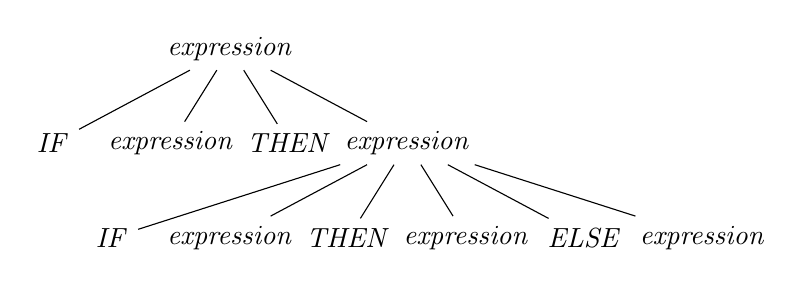
\begin{tikzpicture}[level distance=12mm]
\node { \nt{expression} }
  child { node {\basic{IF}} }
  child { node {\nt{expression}} }
  child { node {\basic{THEN}} }
  child { node {\nt{expression}}
    child { node {\basic{IF}} }
    child { node {\nt{expression}} }
    child { node {\basic{THEN}} }
    child { node {\nt{expression}} }
    child { node {\basic{ELSE}} }
    child { node {\nt{expression}} }
  }
;
\end{tikzpicture}
\end{center}
\caption{A partial derivation tree that justifies shifting}
\label{fig:shifting:tree}
\end{figure}

\begin{figure}
\begin{center}
\begin{tabbing}
\= \nt{expression} \\
\> \basic{IF} \nt{expression} \basic{THEN} \= \nt{expression} \\
\>                                         \> \basic{IF} \nt{expression} \basic{THEN} \basic{expression}
                                              . \basic{ELSE} \nt{expression}
\end{tabbing}
\end{center}
\caption{A textual version of the tree in \fref{fig:shifting:tree}}
\label{fig:shifting:text}
\end{figure}

In our example, the proof that shifting is possible is the derivation tree
shown in Figures~\ref{fig:shifting:tree} and~\ref{fig:shifting:text}. At the
root of the tree is the grammar's start symbol, \nt{expression}. This symbol
develops into the string \nt{IF expression THEN expression}, which forms the
tree's second level. The second occurrence of \nt{expression} in that string
develops into \nt{IF expression THEN expression ELSE expression}, which forms
the tree's last level. The tree's fringe, a sentential form, is the string
\nt{IF expression THEN IF expression THEN expression ELSE expression}. As
announced earlier, it begins with the conflict string \nt{IF expression THEN
IF expression THEN expression}, followed with the conflict token
\nt{ELSE}.

In \fref{fig:shifting:text}, the end of the conflict string is materialized
with a dot. Note that this dot does not occupy the rightmost position in the
tree's last level. In other words, the conflict token (\basic{ELSE}) itself
occurs on the tree's last level. In practical terms, this means that, after
the automaton has recognized the conflict string and peeked at the conflict
token, it makes sense for it to \emph{shift} that token.

\paragraph{Why reducing is legal}

\begin{figure}
\mycommonbaseline
\begin{center}
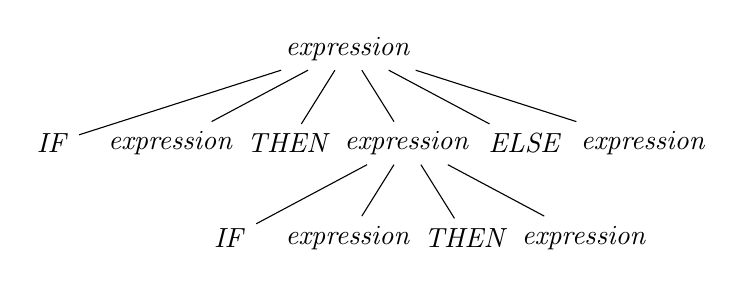
\begin{tikzpicture}[level distance=12mm]
\node { \nt{expression} }
  child { node {\basic{IF}} }
  child { node {\nt{expression}} }
  child { node {\basic{THEN}} }
  child { node {\nt{expression}}
    child { node {\basic{IF}} }
    child { node {\nt{expression}} }
    child { node {\basic{THEN}} }
    child { node {\nt{expression}} }
  }
  child { node {\basic{ELSE}} }
  child { node {\nt{expression}} }
;
\end{tikzpicture}
\end{center}
\caption{A partial derivation tree that justifies reducing}
\label{fig:reducing:tree}
\end{figure}

\begin{figure}
\begin{center}
\begin{tabbing}
\= \nt{expression} \\
\> \basic{IF} \nt{expression} \basic{THEN} \= \nt{expression} \basic{ELSE} \nt{expression}
                                                              \sidecomment{lookahead token appears} \\
\>                                         \> \basic{IF} \nt{expression} \basic{THEN} \basic{expression} .
\end{tabbing}
\end{center}
\caption{A textual version of the tree in \fref{fig:reducing:tree}}
\label{fig:reducing:text}
\end{figure}

In our example, the proof that shifting is possible is the derivation tree
shown in Figures~\ref{fig:reducing:tree} and~\ref{fig:reducing:text}. Again,
the sentential form found at the fringe of the tree begins with the conflict
string, followed with the conflict token.

Again, in \fref{fig:reducing:text}, the end of the conflict string is
materialized with a dot. Note that, this time, the dot occupies the rightmost
position in the tree's last level. In other words, the conflict token
(\basic{ELSE}) appeared on an earlier level (here, on the second level).  This
fact is emphasized by the comment \inlinesidecomment{lookahead token appears}
found at the second level. In practical terms, this means that, after the
automaton has recognized the conflict string and peeked at the conflict token,
it makes sense for it to \emph{reduce} the production that corresponds to the
tree's last level---here, the production is \nt{expression} $\rightarrow$
\basic{IF} \nt{expression} \basic{THEN} \basic{expression}.

\paragraph{An example of a more complex derivation tree}

Figures~\ref{fig:xreducing:tree} and~\ref{fig:xreducing:text} show a partial
derivation tree that justifies reduction in a more complex situation. (This
derivation tree is relative to a grammar that is not shown.) Here, the
conflict string is \basic{DATA UIDENT EQUALS UIDENT}; the conflict token is
\basic{LIDENT}.  It is quite clear that the fringe of the tree begins with the
conflict string.  However, in this case, the fringe does not explicitly
exhibit the conflict token. Let us examine the tree more closely and answer
the question: following \basic{UIDENT}, what's the next terminal symbol on the
fringe?

\begin{figure}
\mycommonbaseline
\begin{center}
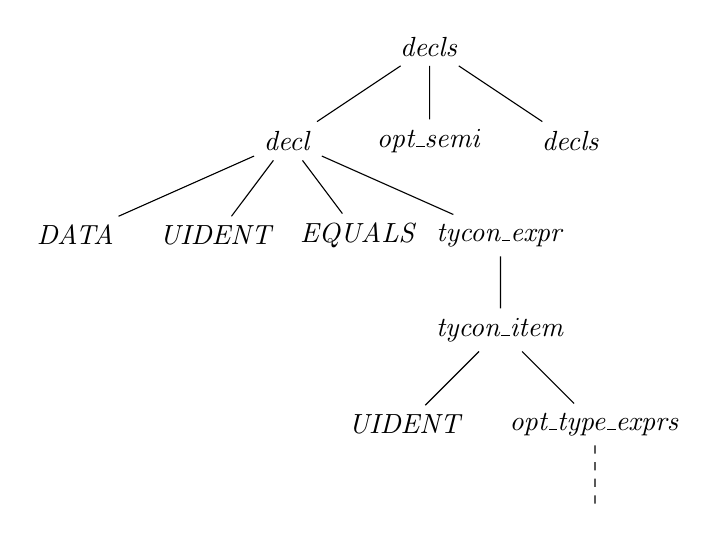
\begin{tikzpicture}[level distance=12mm,level 1/.style={sibling distance=18mm},
                                        level 2/.style={sibling distance=18mm},
                                        level 4/.style={sibling distance=24mm}]]
\node { \nt{decls} }
  child { node {\nt{decl}}
    child { node {\basic{DATA}} }
    child { node {\basic{UIDENT}} }
    child { node {\basic{EQUALS}} }
    child { node {\nt{tycon\_expr}}
      child { node {\nt{tycon\_item}}
        child { node {\basic{UIDENT}} }
        child { node {\nt{opt\_type\_exprs}}
          child { node {} edge from parent [dashed] }
        }
      }
    }
  }
  child { node {\nt{opt\_semi}} }
  child { node {\nt{decls}} }
;    
\end{tikzpicture}
\end{center}
\caption{A partial derivation tree that justifies reducing}
\label{fig:xreducing:tree}
\end{figure}

\begin{figure}
\begin{center}
\begin{tabbing}
\= \nt{decls} \\
\> \nt{decl} \nt{opt\_semi} \nt{decls}
\sidecomment{lookahead token appears because \nt{opt\_semi} can vanish
   and \nt{decls} can begin with \basic{LIDENT}} \\
\> \basic{DATA UIDENT} \basic{EQUALS} \= \nt{tycon\_expr}
\sidecomment{lookahead token is inherited} \\
\> \> \nt{tycon\_item} \sidecomment{lookahead token is inherited} \\
\> \> \basic{UIDENT} \= \nt{opt\_type\_exprs} \sidecomment{lookahead token is inherited} \\
\> \> \> .
\end{tabbing}
\end{center}
\caption{A textual version of the tree in \fref{fig:xreducing:tree}}
\label{fig:xreducing:text}
\end{figure}

First, note that \nt{opt\_type\_exprs} is \emph{not} a leaf node, even though
it has no children. The grammar contains the production $\nt{opt\_type\_exprs}
\rightarrow \epsilon$: the nonterminal symbol \nt{opt\_type\_exprs} develops
to the empty string. (This is made clear in \fref{fig:xreducing:text}, where a
single dot appears immediately below \nt{opt\_type\_exprs}.) Thus,
\nt{opt\_type\_exprs} is not part of the fringe.

Next, note that \nt{opt\_type\_exprs} is the rightmost symbol within its
level. Thus, in order to find the next symbol on the fringe, we have to look
up one level. This is the meaning of the comment \inlinesidecomment{lookahead
token is inherited}. Similarly, \nt{tycon\_item} and \nt{tycon\_expr} appear
rightmost within their level, so we again have to look further up.

This brings us back to the tree's second level. There, \nt{decl} is \emph{not}
the rightmost symbol: next to it, we find \nt{opt\_semi} and \nt{decls}. Does
this mean that \nt{opt\_semi} is the next symbol on the fringe? Yes and no.
\nt{opt\_semi} is a \emph{nonterminal} symbol, but we are really interested in finding
out what the next \emph{terminal} symbol on the fringe could be. The partial
derivation tree shown in Figures~\ref{fig:xreducing:tree}
and~\ref{fig:xreducing:text} does not explicitly answer this question. In
order to answer it, we need to know more about \nt{opt\_semi} and \nt{decls}.

Here, \nt{opt\_semi} stands (as one might have guessed) for an optional
semicolon, so the grammar contains a production $\nt{opt\_semi} \rightarrow
\epsilon$. This is indicated by the comment
\inlinesidecomment{\nt{opt\_semi} can vanish}. (Nonterminal symbols
that generate $\epsilon$ are also said to be \emph{nullable}.) Thus, one could
choose to turn this partial derivation tree into a larger one by developing
\nt{opt\_semi} into $\epsilon$, making it a non-leaf node. That would yield
a new partial derivation tree where the next symbol on the fringe, following
\basic{UIDENT}, is \nt{decls}.

Now, what about \nt{decls}? Again, it is a \emph{nonterminal} symbol, and we
are really interested in finding out what the next \emph{terminal} symbol on
the fringe could be. Again, we need to imagine how this partial derivation
tree could be turned into a larger one by developing \nt{decls}. Here, the
grammar happens to contain a production of the form $\nt{decls} \rightarrow
\basic{LIDENT} \ldots$ This is indicated by the comment
\inlinesidecomment{\nt{decls} can begin with \basic{LIDENT}}.
Thus, by developing \nt{decls}, it is possible to construct a partial
derivation tree where the next symbol on the fringe, following
\basic{UIDENT}, is \basic{LIDENT}. This is precisely the conflict
token.

To sum up, there exists a partial derivation tree whose
fringe begins the conflict string, followed with the conflict token.
Furthermore, in that derivation tree, the dot occupies the rightmost position
in the last level. As in our previous example, this means that, after the
automaton has recognized the conflict string and peeked at the conflict token,
it makes sense for it to \emph{reduce} the production that corresponds to the
tree's last level---here, the production is $\nt{opt\_type\_exprs}
\rightarrow \epsilon$.

\paragraph{Greatest common factor among derivation trees}

Understanding conflicts requires comparing two (or more) derivation trees. It
is frequent for these trees to exhibit a common factor, that is, to exhibit
identical structure near the top of the tree, and to differ only below a
specific node. Manual identification of that node can be tedious, so \menhir
performs this work automatically. When explaining a $n$-way conflict, it first
displays the greatest common factor of the $n$ derivation trees. A question
mark symbol $\basic{(?)}$ is used to identify the node where the trees begin
to differ. Then, \menhir displays each of the $n$ derivation trees,
\emph{without their common factor} -- that is, it displays $n$ sub-trees that
actually begin to differ at the root. This should make visual comparisons
significantly easier.

\subsection{How are severe conflicts resolved in the end?}

It is unspecified how severe conflicts are resolved. \menhir attempts to mimic
\ocamlyacc's specification, that is, to resolve shift/reduce conflicts in favor
of shifting, and to resolve reduce/reduce conflicts in favor of the production
that textually appears earliest in the grammar specification. However, this
specification is inconsistent in case of three-way conflicts, that is,
conflicts that simultaneously involve a shift action and several reduction
actions. Furthermore, textual precedence can be undefined when the grammar
specification is split over multiple modules. In short, \menhir's philosophy is
that
\begin{center}
severe conflicts should not be tolerated,
\end{center}
so you should not care how they are resolved.

% If a shift/reduce conflict is resolved in favor of reduction, then there can
% exist words of terminal symbols that are accepted by the canonical LR(1)
% automaton without traversing any conflict state and which are rejected by our
% automaton (constructed by Pager's method followed by conflict
% resolution). Same problem when a shift/reduce conflict is resolved in favor of
% neither action (via \dnonassoc) or when a reduce/reduce conflict is resolved
% arbitrarily.

\subsection{End-of-stream conflicts}
\label{sec:eos}

\menhir's treatment of the end of the token stream is (believed to be) fully compatible
with \ocamlyacc's. Yet, \menhir attempts to be more user-friendly by warning
about a class of so-called ``end-of-stream conflicts''.

\paragraph{How the end of stream is handled}

In many textbooks on parsing, it is assumed that the lexical analyzer, which
produces the token stream, produces a special token, written \eos, to signal
that the end of the token stream has been reached. A parser generator can take
advantage of this by transforming the grammar: for each start symbol $\nt{S}$
in the original grammar, a new start symbol $\nt{S'}$ is defined, together
with the production $S'\rightarrow S\eos$. The symbol $S$ is no longer a start
symbol in the new grammar. This means that the parser will accept a sentence
derived from $S$ only if it is immediately followed by the end of the token
stream.

This approach has the advantage of simplicity. However, \ocamlyacc and \menhir
do not follow it, for several reasons. Perhaps the most convincing one is that
it is not flexible enough: sometimes, it is desirable to recognize a sentence
derived from $S$, \emph{without} requiring that it be followed by the end of
the token stream: this is the case, for instance, when reading commands, one
by one, on the standard input channel. In that case, there is no end of stream:
the token stream is conceptually infinite. Furthermore, after a command has
been recognized, we do \emph{not} wish to examine the next token, because
doing so might cause the program to block, waiting for more input.

In short, \ocamlyacc and \menhir's approach is to recognize a sentence derived
from $S$ and to \emph{not look}, if possible, at what follows. However, this
is possible only if the definition of $S$ is such that the end of an
$S$-sentence is identifiable without knowledge of the lookahead token. When
the definition of $S$ does not satisfy this criterion, and \emph{end-of-stream
conflict} arises: after a potential $S$-sentence has been read, there can be a
tension between consulting the next token, in order to determine whether the
sentence is continued, and \emph{not} consulting the next token, because the
sentence might be over and whatever follows should not be read. \menhir warns
about end-of-stream conflicts, whereas \ocamlyacc does not.

\paragraph{A definition of end-of-stream conflicts}

Technically, \menhir proceeds as follows. A \eos symbol is introduced. It is,
however, only a \emph{pseudo-}token: it is never produced by the lexical
analyzer. For each start symbol $\nt{S}$ in the original grammar, a new start
symbol $\nt{S'}$ is defined, together with the production $S'\rightarrow S$.
The corresponding start state of the LR(1) automaton is composed of the LR(1)
item $S' \rightarrow . \;S\; [\eos]$. That is, the pseudo-token \eos initially
appears in the lookahead set, indicating that we expect to be done after
recognizing an $S$-sentence. During the construction of the LR(1) automaton,
this lookahead set is inherited by other items, with the effect that, in the
end, the automaton has:
\begin{itemize}
\item \emph{shift} actions only on physical tokens; and
\item \emph{reduce} actions either on physical tokens or on the pseudo-token \eos.
\end{itemize}
A state of the automaton has a reduce action on \eos if, in that state, an
$S$-sentence has been read, so that the job is potentially finished. A state
has a shift or reduce action on a physical token if, in that state, more
tokens potentially need to be read before an $S$-sentence is recognized. If a
state has a reduce action on \eos, then that action should be taken
\emph{without} requesting the next token from the lexical analyzer. On the
other hand, if a state has a shift or reduce action on a physical token, then
the lookahead token \emph{must} be consulted in order to determine if that
action should be taken.

\begin{figure}[p]
\begin{quote}
\begin{tabular}{l}
\dtoken \kangle{\basic{int}} \basic{INT} \\
\dtoken \basic{PLUS TIMES} \\
\dleft PLUS \\
\dleft TIMES \\
\dstart \kangle{\basic{int}} \nt{expr} \\
\percentpercent \\
\nt{expr}:
\newprod \basic{i} = \basic{INT} \dpaction{\basic{i}}
\newprod \basic{e1} = \nt{expr} \basic{PLUS} \basic{e2} = \nt{expr} \dpaction{\basic{e1 + e2}}
\newprod \basic{e1} = \nt{expr} \basic{TIMES} \basic{e2} = \nt{expr} \dpaction{\basic{e1 * e2}}
\end{tabular}
\end{quote}
\caption{Basic example of an end-of-stream conflict}
\label{fig:basiceos}
\end{figure}

\begin{figure}[p]
\begin{verbatim}
State 6:
expr -> expr . PLUS expr [ # TIMES PLUS ]
expr -> expr PLUS expr . [ # TIMES PLUS ]
expr -> expr . TIMES expr [ # TIMES PLUS ]
-- On TIMES shift to state 3
-- On # PLUS reduce production expr -> expr PLUS expr 

State 4:
expr -> expr . PLUS expr [ # TIMES PLUS ]
expr -> expr . TIMES expr [ # TIMES PLUS ]
expr -> expr TIMES expr . [ # TIMES PLUS ]
-- On # TIMES PLUS reduce production expr -> expr TIMES expr 

State 2:
expr' -> expr . [ # ]
expr -> expr . PLUS expr [ # TIMES PLUS ]
expr -> expr . TIMES expr [ # TIMES PLUS ]
-- On TIMES shift to state 3
-- On PLUS shift to state 5
-- On # accept expr
\end{verbatim}
\caption{Part of an LR automaton for the grammar in \fref{fig:basiceos}}
\label{fig:basiceosdump}
\end{figure}

\begin{figure}[p]
\begin{quote}
\begin{tabular}{l}
\ldots \\
\dtoken \basic{END} \\
\dstart \kangle{\basic{int}} \nt{main} \hskip 1cm \textit{// instead of \nt{expr}} \\
\percentpercent \\
\nt{main}:
\newprod \basic{e} = \nt{expr} \basic{END} \dpaction{\basic{e}} \\
\nt{expr}:
\newprod \ldots
\end{tabular}
\end{quote}
\caption{Fixing the grammar specification in \fref{fig:basiceos}}
\label{fig:basiceos:sol}
\end{figure}

An end-of-stream conflict arises when a state has distinct actions on \eos and
on at least one physical token. In short, this means that the end of an
$S$-sentence cannot be unambiguously identified without examining one extra
token. \menhir's default behavior, in that case, is to suppress the action on
\eos, so that more input is \emph{always} requested.

\paragraph{Example}

\fref{fig:basiceos} shows a grammar that has end-of-stream conflicts.
When this grammar is processed, \menhir warns about these conflicts,
and further warns that \nt{expr} is never accepted. Let us explain.

Part of the corresponding automaton, as described in the \conflicts file, is
shown in \fref{fig:basiceosdump}. Explanations at the end of the \conflicts
file (not shown) point out that states 6 and 2 have an end-of-stream
conflict. Indeed, both states have distinct actions on \eos and on the
physical token \basic{TIMES}.
%
It is interesting to note that, even though state 4 has actions on \eos and on
physical tokens, it does not have an end-of-stream conflict. This is because
the action taken in state 4 is always to reduce the production $\nt{expr}
\rightarrow \nt{expr}$ \basic{TIMES} \nt{expr}, regardless of the lookahead
token.

By default, \menhir produces a parser where end-of-stream conflicts are
resolved in favor of looking ahead: that is, the problematic reduce actions on
\eos are suppressed. This means, in particular, that the \emph{accept} action
in state 2, which corresponds to reducing the production $\nt{expr}
\rightarrow \nt{expr'}$, is suppressed. This explains why the symbol \nt{expr}
is never accepted: because expressions do not have an unambiguous end marker,
the parser will always request one more token and will never stop.

In order to avoid this end-of-stream conflict, the standard solution is to
introduce a new token, say \basic{END}, and to use it as an end marker for
expressions. The \basic{END} token could be generated by the lexical analyzer
when it encounters the actual end of stream, or it could correspond to a piece
of concrete syntax, say, a line feed character, a semicolon, or an
\texttt{end} keyword. The solution is shown in \fref{fig:basiceos:sol}.

% ---------------------------------------------------------------------------------------------------------------------

\section{Positions}
\label{sec:positions}

When an \ocamllex-generated lexical analyzer produces a token, it updates
two fields, named \verb+lex_start_p+ and \verb+lex_curr_p+, in its environment
record, whose type is \verb+Lexing.lexbuf+. Each of these fields holds a value
of type \verb+Lexing.position+. Together, they represent the token's start and
end positions within the text that is being scanned. A position consists
mainly of an offset (the position's \verb+pos_cnum+ field), but also holds
information about the current file name, the current line number, and the
current offset within the current line. (Not all \ocamllex-generated analyzers
keep this extra information up to date. This must be explicitly programmed by
the author of the lexical analyzer.)

\begin{figure}
\begin{center}
\begin{tabular}{lp{9cm}}
\verb+$startpos+ & start position of the sentence derived out of the production that is being reduced \\
\verb+$endpos+   & end position of the sentence derived out of the production that is being reduced \\
\verb+$startpos(+ \verb+$+\nt{i} \barre \nt{id} \verb+)+
                 & start position of the sentence derived out of the symbol whose semantic value is referred to as
                   \verb+$+\nt{i} or \nt{id} \\
\verb+$endpos(+ \verb+$+\nt{i} \barre \nt{id} \verb+)+
                 & end position of the sentence derived out of the symbol whose semantic value is referred to as
                   \verb+$+\nt{i} or \nt{id} \\
\verb+$startofs+ & start offset of the sentence derived out of the production that is being reduced \\
\verb+$endofs+   & end offset of the sentence derived out of the production that is being reduced \\
\verb+$startofs(+ \verb+$+\nt{i} \barre \nt{id} \verb+)+
                 & start offset of the sentence derived out of the symbol whose semantic value is referred to as
                   \verb+$+\nt{i} or \nt{id} \\
\verb+$endofs(+ \verb+$+\nt{i} \barre \nt{id} \verb+)+
                 & end offset of the sentence derived out of the symbol whose semantic value is referred to as
                   \verb+$+\nt{i} or \nt{id} \\
\end{tabular}
\end{center}
\caption{Position-related keywords}
\label{fig:pos}
\end{figure}

This mechanism allows associating pairs of positions with terminal symbols. If
desired, \menhir automatically extends it to nonterminal symbols as well. That
is, it offers a mechanism for associating pairs of positions with terminal or
nonterminal symbols. This is done by making a set of keywords, documented in
\fref{fig:pos}, available to semantic actions. Note that these keywords are
\emph{not} available elsewhere---in particular, not within \ocaml headers.
Note also that \ocaml's standard library module \texttt{Parsing} is
deprecated. The functions that it offers \emph{can} be called, but will return
dummy positions.

% ---------------------------------------------------------------------------------------------------------------------

\section{Error handling}
\label{sec:errors}

\paragraph{Error handling}

\menhir's error handling mechanism is inspired by that of \yacc and
\ocamlyacc, but is not identical. A special \error token is made available
for use within productions. The LR automaton is constructed exactly as if
\error was a regular terminal symbol. However, \error is never produced
by the lexical analyzer. Instead, when an error is detected, the current
lookahead token is discarded and replaced with the \error token, which becomes
the current lookahead token. At this point, the parser enters \emph{error
handling} mode.

In error handling mode, automaton states are popped off the automaton's stack
until a state that can \emph{act} on \error is found. This includes
\emph{both} shift \emph{and} reduce actions. (\yacc and \ocamlyacc do not
trigger reduce actions on \error. It is somewhat unclear why this is so.)

When a state that can reduce on \error is found, reduction is performed.
Since the lookahead token is still \error, the automaton remains in error
handling mode.

When a state that can shift on \error is found, the \error token is shifted.
At this point, the parser returns to normal mode.

When no state that can act on \error is found on the automaton's stack, the
parser stops and raises the exception \texttt{Error}. This exception carries
no information. The position of the error can be obtained by reading the
lexical analyzer's environment record.

\paragraph{Error recovery}

\ocamlyacc offers an error recovery mode, which is entered immediately after
an \error token was successfully shifted. In this mode, tokens are repeatedly
taken off the input stream and discarded until an acceptable token is found.
This feature is no longer offered by \menhir.

\paragraph{Error-related keywords}

The following keyword is made available to semantic actions.

When the \verb+$syntaxerror+ keyword is evaluated, evaluation of the semantic
action is aborted, so that the current reduction is abandoned; the current
lookahead token is discarded and replaced with the \error token; and error
handling mode is entered.  Note that there is no mechanism for inserting an
\error token \emph{in front of} the current lookahead token, even though this
might also be desirable.  It is unclear whether this keyword is useful; it
might be suppressed in the future.

\paragraph{When are errors detected?}

An error is detected when the current state of the automaton has no action on
the current lookahead token. Thus, understanding exactly when errors are
detected requires understanding how the automaton is constructed. \menhir's
construction technique is \emph{not} Knuth's canonical LR(1)
technique~\cite{knuth-lr-65}, which is too expensive to be practical. Instead,
\menhir \emph{merges} states~\cite{pager-77} and introduces so-called \emph{default
reductions}. Both techniques can \emph{defer} error detection by allowing
extra reductions to take place before an error is detected. All LALR(1) parser
generators exhibit the same problem.

% ---------------------------------------------------------------------------------------------------------------------

\section{Using \menhir as an interpreter}
\label{sec:interpret}

When \ointerpret is set, \menhir no longer behaves as a compiler. Instead,
it acts as an interpreter. That is, it repeatedly:
\begin{itemize}
\item reads a sentence off the standard input channel;
\item parses this sentence, according to the grammar;
\item displays an outcome.
\end{itemize}
This process stops when the end of the input channel is reached.

\subsection{Sentences}
\label{sec:sentences}

The syntax of sentences is as follows:
\begin{center}
\begin{tabular}{r@{}c@{}l}
\nt{sentence} \is
  \optional{\nt{lid}\,\deuxpoints} \sepspacelist{\nt{uid}} \,\dnewline
\end{tabular}
\end{center}

Less formally, a sentence is a sequence of zero or more terminal symbols
(\nt{uid}'s), separated with whitespace, terminated with a newline character,
and optionally preceded with a non-terminal start symbol (\nt{lid}). This
non-terminal symbol can be omitted if, and only if, the grammar only has one
start symbol.

For instance, here are four valid sentences for the grammar of arithmetic
expressions found in the directory \distrib{demos/calc}:
%
\begin{verbatim}
main: INT PLUS INT EOL
INT PLUS INT
INT PLUS PLUS INT EOL
INT PLUS PLUS
\end{verbatim}
%
In the first sentence, the start symbol \texttt{main} was explicitly
specified. In the other sentences, it was omitted, which is permitted, because
this grammar has no start symbol other than \texttt{main}.  The first sentence
is a stream of four terminal symbols, namely \texttt{INT}, \texttt{PLUS},
\texttt{INT}, and \texttt{EOL}. These terminal symbols must be provided under
their symbolic names. Writing, say, ``\texttt{12+32\textbackslash n}'' instead
of \texttt{INT PLUS INT EOL} is not permitted. \menhir would not be able to
make sense of such a concrete notation, since it does not have a lexer for it.

% On pourrait documenter le fait qu'une phrase finie est transform�e par Menhir
% en un flot de tokens potentiellement infinie, avec un suffixe infini EOF ...
% Mais c'est un hack, qui pourrait changer � l'avenir.

\subsection{Outcomes}
\label{sec:outcomes}

As soon as \menhir is able to read a complete sentence off the standard input
channel (that is, as soon as it finds the newline character that ends the
sentence), it parses the sentence according to whichever grammar was specified
on the command line, and displays an outcome.

An outcome is one of the following:
\begin{itemize}
\item \texttt{ACCEPT}: a prefix of the sentence was successfully parsed;
      a parser generated by \menhir would successfully stop and produce
      a semantic value;
\item \texttt{OVERSHOOT}: the end of the sentence was reached before it
      could be accepted; a parser generated by \menhir would request a
      non-existent ``next token'' from the lexer, causing it to fail or
      block;
\item \texttt{REJECT}: the sentence was not accepted; a parser generated
      by \menhir would raise the exception \texttt{Error}.
\end{itemize}

When \ointerpretshowcst is set, each \texttt{ACCEPT} outcome is followed with
a concrete syntax tree. A concrete syntax tree is either a leaf or a node.  A
leaf is either a terminal symbol or \error. A node is annotated with a
non-terminal symbol, and carries a sequence of immediate descendants that
correspond to a valid expansion of this non-terminal symbol. \menhir's
notation for concrete syntax trees is as follows:
\begin{center}
\begin{tabular}{r@{}c@{}l}
\nt{cst} \is
   \nt{uid} \\
&& \error \\
&& \texttt{[} \nt{lid}\,\deuxpoints \sepspacelist{\nt{cst}} \texttt{]}
\end{tabular}
\end{center}

% This notation is not quite unambiguous (it is ambiguous if several
% productions are identical).

For instance, if one wished to parse the example sentences of
\sref{sec:sentences} using the grammar of arithmetic expressions in
\distrib{demos/calc}, one could invoke \menhir as follows:
\begin{verbatim}
$ menhir --interpret --interpret-show-cst demos/calc/parser.mly
main: INT PLUS INT EOL
ACCEPT
[main: [expr: [expr: INT] PLUS [expr: INT]] EOL]
INT PLUS INT
OVERSHOOT
INT PLUS PLUS INT EOL
REJECT
INT PLUS PLUS
REJECT
\end{verbatim}
(Here, \menhir's input---the sentences provided by the user on the standard
input channel--- is shown intermixed with \menhir's output---the outcomes
printed by \menhir on the standard output channel.) The first sentence is
valid, and accepted; a concrete syntax tree is displayed. The second sentence
is incomplete, because the grammar specifies that a valid expansion of
\texttt{main} ends with the terminal symbol \texttt{EOL}; hence, the outcome
is \texttt{OVERSHOOT}. The third sentence is invalid, because of the repeated
occurrence of the terminal symbol \texttt{PLUS}; the outcome is
\texttt{REJECT}. The fourth sentence, a prefix of the third one, is rejected
for the same reason.

\subsection{Remarks}

Using \menhir as an interpreter offers an easy way of debugging your grammar.
For instance, if one wished to check that addition is considered
left-associative, as requested by the \dleft directive found in the file
\distrib{demos/calc/parser.mly}, one could submit the following sentence:
\begin{verbatim}
$ ./menhir --interpret --interpret-show-cst ../demos/calc/parser.mly
INT PLUS INT PLUS INT EOL
ACCEPT
[main:
  [expr: [expr: [expr: INT] PLUS [expr: INT]] PLUS [expr: INT]]
  EOL
]
\end{verbatim}
%$
The concrete syntax tree displayed by \menhir is skewed towards the left,
as desired.

The switches \ointerpret and \otrace can be used in conjunction. When
\otrace is set, the interpreter logs its actions to the standard error
channel.

% ---------------------------------------------------------------------------------------------------------------------

\section{Generated API}

\newcommand{\mystartsymbol}{\texttt{main}\xspace}
\newcommand{\mystartsymboltype}{\texttt{thing}\xspace}

When \menhir processes a grammar specification, say \texttt{parser.mly}, it
produces one \ocaml module, \texttt{Parser}, whose code resides in the file
\texttt{parser.ml} and whose signature resides in the file
\texttt{parser.mli}. We now review this signature.
We assume that the grammar specification has just one start symbol
\mystartsymbol, whose \ocaml type is \mystartsymboltype. 

% On passe sous silence la d�finition du type token, qui peut �tre absente
% ou pr�sente, et est expliqu�e ailleurs.

\subsection{Monolithic API}
\label{sec:monolithic}

The monolithic API consists in just one parsing function, named after the
start symbol:
\begin{verbatim}
  val main: (Lexing.lexbuf -> token) -> Lexing.lexbuf -> thing
\end{verbatim}
% On ne montre pas la d�finition de l'exception Error.
This function expects two arguments, namely: a lexer, which typically is produced by
\ocamllex and has type \verb+Lexing.lexbuf -> token+; and a lexing buffer,
which has type \verb+Lexing.lexbuf+. This API is compatible with
\ocamlyacc. (For information on using \menhir without \ocamllex, please
consult \sref{sec:qa}.)
%
This API is ``monolithic'' in the sense that there is just one function, which
does everything: it pulls tokens from the lexer, parses, and eventually
returns a semantic value (or fails by throwing the exception \texttt{Error}).

\subsection{Incremental API}
\label{sec:incremental}

If \otable is set, \menhir offers an incremental API in addition to the
monolithic API. In this API, control is inverted. The parser does not have
access to the lexer. Instead, when the parser needs the next token, it stops
and returns its current state to the user. The user is then responsible for
obtaining this token (typically by invoking the lexer) and resuming the parser
from that state.

This API is ``incremental'' in the sense that the user has access to a
sequence of the intermediate states of the parser. Assuming that semantic
values are immutable, a parser state is a persistent data structure: it can be
stored and used multiple times, if desired. This enables applications such as
``live parsing'', where a buffer is continuously parsed while it is being
edited. The parser can be re-started in the middle of the buffer whenever the
user edits a character. Because two successive parser states share most of
their data in memory, a list of $n$ successive parser states occupies only
$O(n)$ space in memory.

% One could point out that semantic actions should be side-effect free.
% But that is an absolute requirement. Semantic actions can have side
% effects, if the user knows what they are doing.

In this API, the parser is started by invoking \verb+main_incremental+,
where \mystartsymbol is the name of the start symbol:
\begin{verbatim}
  val main_incremental: unit -> thing MenhirInterpreter.result
\end{verbatim}

The sub-module \menhirinterpreter is also part of the incremental API.
Its declaration, which appears in the file \texttt{parser.mli}, is as
follows:
\begin{verbatim}
  module MenhirInterpreter : MenhirLib.IncrementalEngine.INCREMENTAL_ENGINE
    with type token := token
\end{verbatim}
The signature \verb+INCREMENTAL_ENGINE+, defined in the module
\menhirlibincrementalengine, contains the following elements.
Please keep in mind that, from the outside, these elements should be referred
to with an appropriate prefix: e.g., the type \verb+result+ should be referred
to as \verb+MenhirInterpreter.result+, or
\verb+Parser.MenhirInterpreter.result+, depending on which modules the user
chooses to open.

\begin{verbatim}
  type 'a result =
    | InputNeeded of ('a, input_needed) env
    | HandlingError of ('a, handling_error) env
    | Accepted of 'a
    | Rejected
\end{verbatim}

The type \verb+'a result+ represents an intermediate or
final result of the parser. An intermediate result is a suspension: it records
the parser's current state, and allows parsing to be resumed. The parameter
\verb+'a+ is the type of the semantic value that will eventually be produced
if the parser succeeds.

\verb+Accepted+ and \verb+Rejected+ are final results. \verb+Accepted+ carries
a semantic value.

\verb+InputNeeded+ is an intermediate result. It means that the parser wishes
to read one token before continuing.

\verb+HandlingError+ is also an intermediate result. It means that the parser
has detected an error and is currently handling it, in several steps. It does
not need more input at this point. The parser suspends itself at this point
only in order to give the user an opportunity to handle this error in a
different manner, if desired.

\begin{verbatim}
  type ('a, 'pc) env
\end{verbatim}

The abstract type \verb+('a, 'pc) env+ represents the current state of the
parser. (That is, it contains the current state and stack of the LR
automaton.) Assuming that semantic values are immutable, it is a persistent
data structure: it can be stored and used multiple times, if desired. The
parameter \verb+'a+ is the type of the semantic value that will eventually be
produced if the parser succeeds. The parameter \verb+'pc+ prevents confusion
between several kinds of intermediate results.

\begin{verbatim}
  val offer:
    ('a, input_needed) env ->
    token * Lexing.position * Lexing.position ->
    'a result
\end{verbatim}

The function \verb+offer+ allows the user to resume the parser after the
parser has suspended itself with a result of the form \verb+InputNeeded env+.
This function expects the parser state \verb+env+ as well as a new token
(together with the start and end positions of this token). It produces a new
result, which again can be an intermediate result or a final result. It does
not raise any exception. (The exception \texttt{Error} is used only in the
monolithic API.)

\begin{verbatim}
   val handle:
    ('a, handling_error) env ->
    'a result
\end{verbatim}

The function \verb+handle+ allows the user to resume the parser after the
parser has suspended itself with a result of the form \verb+HandlingError env+.
This function expects just the parser state \verb+env+. It produces a new
result. It does not raise any exception.

The incremental API subsumes the monolithic API. Indeed, \verb+main+ can
be (and is in fact) implemented by first calling \verb+main_incremental+, then
calling \verb+offer+ and \verb+handle+ in a loop, until a final result is
obtained.

At this time, because the type \verb+('a, 'pc) env+ is opaque, the state of
the parser cannot be inspected by the user. We plan to offer an inspection API
in the near future.

% ---------------------------------------------------------------------------------------------------------------------

\section{Coq back-end}
\label{sec:coq}

\menhir is able to generate a parser that whose correctness can be formally
verified using the Coq proof assistant~\cite{jourdan-leroy-pottier-12}. This
feature is used to construct the parser of the CompCert certified C
compiler~\cite{compcert}.

Setting the \ocoq switch on the command line enables the Coq back-end.  When
this switch is set, \menhir expects an input file whose name ends
in \texttt{.vy} and generates a Coq file whose name ends
in \texttt{.v}.

Like a \texttt{.mly} file, a \texttt{.vy} file is a grammar specification,
with embedded semantic actions. The main difference is that the semantic
actions in a \texttt{.vy} file are expressed in Coq instead
of \ocaml. A \texttt{.vy} file otherwise uses the same syntax as
a \texttt{.mly} file. There are however several restrictions:
%
\begin{itemize}
\item The error handling mechanism (\sref{sec:errors}) is absent.
      The \verb+$syntaxerror+ keyword and the \error token are not supported.
\item Location information is not propagated. The \verb+$start*+ and \verb+$end*+
      keywords (\fref{fig:pos}) are not supported.
\item \dparameter (\sref{sec:parameter}) is not supported.
\item \dinline (\sref{sec:inline}) is not supported.
\item The standard library (\sref{sec:library}) is not supported, of course,
      because its semantic actions are expressed in \ocaml. If desired, the user can define
      an analogous library, whose semantic actions are expressed in Coq.
\item Because Coq's type inference algorithm is rather unpredictable,
      the Coq type of every nonterminal symbol must be provided via a
      \dtype or \dstart declaration (\sref{sec:type}, \sref{sec:start}).
\item Unless the proof of completeness has been deactivated using
  \ocoqnocomplete, the grammar must not have a conflict
  (not even a benign one, in the sense of \sref{sec:conflicts:benign}).
  That is, the grammar must be LR(1). Conflict resolution via
  priority and associativity declarations (\sref{sec:assoc})
  is not supported.
  The reason is that there is no simple formal specification
  of how conflict resolution should work.
\end{itemize}

The generated file contains several modules:

\begin{itemize}
\item The module \verb+Gram+ defines the terminal and
  non-terminal symbols, the grammar, and the semantic actions.
\item The module \verb+Aut+ contains the automaton
  generated by \menhir, together with a certificate that is checked by Coq
  while establishing the soundness and completeness of the parser.
\end{itemize}

The type of the terminal symbols is an inductive type, with one constructor
for each terminal symbol. A~terminal symbol per se does not carry a the
semantic value. We also define the type \verb+token+ of tokens, i.e.,
dependent pairs of a terminal symbol and a semantic value of an appropriate
type for this symbol. We model the lexer as an object of type
\verb+Streams.Stream token+, i.e., an infinite stream of tokens.

The proof of termination of an LR(1) parser in the case of invalid input seems
far from obvious. We did not find such a proof in the literature. In an
application such as CompCert~\cite{compcert}, this question is not considered
crucial. For this reason, we did not formally establish the termination of the
parser. Instead, we use the ``fuel'' technique. The parser takes an additional
parameter of type \verb+nat+ that indicates the maximum number of steps the
parser is allowed to perform. In practice, after extracting the code to
\ocaml, one can use the standard trick of passing an infinite amount of fuel,
defined in \ocaml by \verb+let rec inf = S inf+.

Parsing can have three different outcomes, represented by the type
\verb+parse_result+.
%
(This definition is implicitly parameterized over the initial
state~\verb+init+. We omit the details here.)
%
\begin{verbatim}
  Inductive parse_result :=
  | Fail_pr:    parse_result
  | Timeout_pr: parse_result
  | Parsed_pr:
      symbol_semantic_type (NT (start_nt init)) ->
      Stream token ->
      parse_result.
\end{verbatim}

The outcome \verb+Fail_pr+ means that parsing has failed because of a syntax
error. (If the completeness of the parser with respect to the grammar has been
proved, this implies that the input is invalid). The outcome \verb+Timeout_pr+
means that the fuel has been exhausted. Of course, this cannot happen if the
parser was given an infinite amount of fuel, as suggested above. The outcome
\verb+Parsed_pr+ means that the parser has succeeded in parsing a prefix of
the input stream. It carries the semantic value that has been constructed for
this prefix, as well as the remainder of the input stream.

For each entry point \verb+entry+ of the grammar, \menhir generates a
parsing function \verb+entry+, whose type is
\verb+nat -> Stream token -> parse_result+.

% jh: Je suis un peu emb�t�, parce que init est
% en r�alit� de type initstate, mais je n'ai pas envie d'en parler
% dans la doc. Tout ce qui importe, c'est que le premier param�tre de
% Parsed_pr a un type compatible avec le type que l'utilisateur a
% donn�.

Two theorems are provided, named \verb+entry_point_correct+ and
\verb+entry_point_complete+. The correctness theorem states that, if a word (a
prefix of the input stream) is accepted, then this word is valid (with respect
to the grammar) and the semantic value that is constructed by the parser is
valid as well (with respect to the grammar). The completeness theorem states
that if a word (a prefix of the input stream) is valid (with respect to the
grammar), then (given sufficient fuel) it is accepted by the parser.

These results imply that the grammar is unambiguous: for every input, there is
at most one valid interpretation. This is proved by another generated theorem,
named \verb+unambiguous+.

% jh: Pas besoin de prouver la terminaison pour avoir la non-ambigu�t�, car
% les cas de non-terminaison ne concernent que les entr�es invalides.
% fp: bien vu!

% fp: ce serait int�ressant d'avoir un certificat comme quoi la grammaire est
% bien LR(1), mais peut-�tre qu'on s'en fout. C'est bien de savoir qu'elle
% est non-ambigu�.

% jh: Je ne sais pas ce que c'est qu'un certificat comme quoi la grammaire
% est LR(1), en pratique...
% fp: Ce serait une preuve d'un th�or�me, exprim� uniquement en termes de
% la grammaire, comme quoi la grammaire est LR(1). Il y a une d�finition
% de cette propri�t� dans le textbook de Aho et Ullman, si je me rappelle
% bien. Mais peu importe.

% fp: On pourrait aussi souhaiter un th�or�me comme quoi le parser ne lit
% pas le stream trop loin...

% jh: pour vraiment prouver cela, il faudrait inverser le
% controle. Sinon, comme r�sultat un peu moins fort, dans la version
% actuelle, on renvoie le stream restant, et on prouve qu'il
% correspond bien � la fin du Stream.

The parsers produced by \menhir's Coq back-end must be linked with a Coq
library, which can be found in the CompCert tree~\cite{compcert}, in the
\verb+cparser/validator+ subdirectory. Additionally, CompCert can be used as
an example if one wishes to use \menhir to generate a formally verified parser
as part of some other project.

% fp: ce pourrait �tre bien de documenter les directives n�cessaires pour
% extraire du code efficace. D'apr�s Xavier ce morceau de extraction.v
% est pertinent:
\begin{comment}
(* Int31 *)
Extract Inductive Int31.digits => "bool" [ "false" "true" ].
Extract Inductive Int31.int31 => "int" [ "Camlcoq.Int31.constr" ] "Camlcoq.Int31.destr".
Extract Constant Int31.twice => "Camlcoq.Int31.twice".
Extract Constant Int31.twice_plus_one => "Camlcoq.Int31.twice_plus_one".
Extract Constant Int31.compare31 => "Camlcoq.Int31.compare".
Extract Constant Int31.On => "0".
Extract Constant Int31.In => "1".
\end{comment}

% ---------------------------------------------------------------------------------------------------------------------

\section{Comparison with \ocamlyacc}

Here is an incomplete list of the differences between \ocamlyacc and \menhir.
The list is roughly sorted by decreasing order of importance.

\begin{itemize}

\item \menhir allows the definition of a nonterminal symbol to be parameterized by other
      (terminal or nonterminal) symbols (\sref{sec:templates}). Furthermore, it offers a library of
      standard parameterized definitions (\sref{sec:library}), including options,
      sequences, and lists. It offers some support for EBNF syntax,
      via the \dquestion, \dplus, and \dstar modifiers.

\item \ocamlyacc only accepts LALR(1) grammars. \menhir accepts LR(1) grammars,
      thus avoiding certain artificial conflicts.

\item \menhir's \dinline keyword (\sref{sec:inline}) helps avoid or resolve some LR(1)
      conflicts without artificial modification of the grammar.

\item \menhir explains conflicts (\sref{sec:conflicts}) in terms of the grammar,
      not just in terms of the automaton. \menhir's explanations are believed
      to be understandable by mere humans.

\item \menhir offers an incremental API (in \otable mode only) (\sref{sec:incremental}). This
          means that the state of the parser can be saved at any point (at no
          cost) and that parsing can later be resumed from a saved state.

\item In \ocoq mode, \menhir produces a parser whose correctness and
  completeness with respect to the grammar can be checked by Coq (\sref{sec:coq}).

\item \menhir offers an interpreter (\sref{sec:interpret}) that helps debug
      grammars interactively.

\item \menhir allows grammar specifications to be split over multiple files (\sref{sec:split}).
      It also allows several grammars to share a single set of tokens.

\item \menhir produces reentrant parsers.

\item \menhir is able to produce parsers that are parameterized by \ocaml
      modules.

\item \ocamlyacc requires semantic values to be referred to via keywords: \verb+$1+,
      \verb+$2+, and so on. \menhir allows semantic values to be explicitly named.

\item \menhir warns about end-of-stream conflicts (\sref{sec:eos}), whereas
      \ocamlyacc does not. \menhir warns about productions that are never
      reduced, whereas, at least in some cases, \ocamlyacc does not.

\item \menhir offers an option to typecheck semantic actions \emph{before}
      a parser is generated: see \oinfer.

\item \ocamlyacc produces tables that are interpreted by a piece of C code,
      requiring semantic actions to be encapsulated as \ocaml closures and
      invoked by C code. \menhir offers a choice between producing tables
      and producing code. In either case, no C code is involved.

\item \menhir makes \ocaml's standard library module \texttt{Parsing}
      entirely obsolete. Access to locations is now via keywords
      (\sref{sec:positions}).  Uses of \verb+raise Parse_error+ within
      semantic actions are deprecated.  The function \verb+parse_error+ is
      deprecated. They are replaced with keywords (\sref{sec:errors}).

\item \menhir's error handling mechanism (\sref{sec:errors}) is inspired
      by \ocamlyacc's, but are not guaranteed to be fully
      compatible. Error recovery, also known as re-synchronization, is not
      supported by \menhir.

\item The way in which severe conflicts (\sref{sec:conflicts}) are resolved
      is not guaranteed to be fully compatible with \ocamlyacc.

\item \menhir warns about unused \dtoken, \dnonassoc, \dleft, and \dright
      declarations. It also warns about \dprec annotations that do not
      help resolve a conflict.

\item \menhir accepts \ocaml-style comments.

\item \menhir allows \dstart and \dtype declarations to be condensed.

\item \menhir allows two (or more) productions to share a single semantic action.

\item \menhir produces better error messages when a semantic action
      contains ill-balanced parentheses.

% \item \ocamlyacc allows nonterminal start symbols to start with an uppercase
%       letter, and produces invalid \ocaml code in that case. \menhir disallows this.

\item \ocamlyacc ignores semicolons and commas everywhere. \menhir also ignores
      semicolons everywhere, but treats commas as significant. Commas are optional
      within \dtoken declarations.

% \item \ocamlyacc ignores multiple definitions of a token, even when two of them are at
%       different types. \menhir rejects this.

\item \ocamlyacc allows \dtype declarations to refer to terminal or non-terminal
      symbols, whereas \menhir requires them to refer to non-terminal symbols.
      Types can be assigned to terminal symbols with a \dtoken declaration.

\end{itemize}

% ---------------------------------------------------------------------------------------------------------------------

\section{Questions and Answers}
\label{sec:qa}

$\mathstrut$ % Ensure correct indentation of the first question. Ugly.

\vspace{-\baselineskip}

\question{Is \menhir faster than \ocamlyacc? What is the speed difference
  between \texttt{menhir} and \texttt{menhir -{}-table}?} A (not quite
scientific) benchmark suggests that the parsers produced by \ocamlyacc and
\texttt{menhir -{}-table} have comparable speed, whereas those produced by
\texttt{menhir} are between 2 and 4 times faster. This benchmark excludes the
time spent in the lexer and in the semantic actions.

\question{Turning on \oinfer broke my \Makefile! What should I do?}
Look at \distrib{demos/Makefile.shared}. It is meant to be re-used
without change. If it does not suit your needs, you can copy parts
of it into your own \Makefile, or submit suggestions for improvement.

\question{I am unable to write a correct \Makefile for \menhir, and so are
  you.} True enough. Have a look at \ocamlbuild. It has built-in compilation
rules for \ocaml and \menhir. That should help.

\question{\menhir reports \emph{more} shift/reduce conflicts than
\ocamlyacc! How come?} \ocamlyacc sometimes merges two states
of the automaton that \menhir considers distinct. This happens
when the grammar is not LALR(1). If these two states happen to
contain a shift/reduce conflict, then \menhir reports two conflicts,
while \ocamlyacc only reports one. Of course, the two conflicts are
very similar, so fixing one will usually fix the other as well.

\question{I do not use \ocamllex. Is there an API that does not involve lexing
  buffers?} Like \ocamlyacc, \menhir produces parsers whose monolithic API
(\sref{sec:monolithic}) is intended for use with \ocamllex. However, it is
possible to convert them, after the fact, to a simpler, revised API. In the
revised API, there are no lexing buffers, and a lexer is just a function from
unit to tokens. Converters are provided by the library module
\menhirlibconvert. This can be useful, for instance, for users of
\texttt{ulex}, the Unicode lexer generator. Also, please note that \menhir's
incremental API (\sref{sec:incremental}) does not mention the type
\verb+Lexing.lexbuf+. In this API, the parser expects to be supplied with
triples of a token and start/end positions of type \verb+Lexing.position+.

% ---------------------------------------------------------------------------------------------------------------------

\section{Technical background}

After experimenting with Knuth's canonical LR(1) technique~\cite{knuth-lr-65},
we found that it \emph{really} is not practical, even on today's computers.
For this reason, \menhir implements a slightly modified version of Pager's
algorithm~\cite{pager-77}, which merges states on the fly if it can be proved
that no reduce/reduce conflicts will arise as a consequence of this
decision. This is how \menhir avoids the so-called \emph{mysterious} conflicts
created by LALR(1) parser generators~\cite[section 5.7]{bison}.

\menhir's algorithm for explaining conflicts is inspired by DeRemer and
Pennello's~\cite{deremer-pennello-82} and adapted for use with Pager's
construction technique.

By default, \menhir produces code, as opposed to tables. This approach has
been explored before~\cite{bhamidipaty-proebsting-98,horspool-faster-90}.
\menhir performs some static analysis of the automaton in order to produce
more compact code.

When asked to produce tables, \menhir performs compression via first-fit
row displacement, as described by Tarjan and Yao~\cite{tarjan-yao-79}.
Double displacement is not used. The action table is made sparse by
factoring out an error matrix, as suggested by Dencker, D�rre, and
Heuft~\cite{dencker-84}.

The type-theoretic tricks that triggered our interest in LR
parsers~\cite{pottier-regis-gianas-typed-lr} are not implemented in \menhir.
In the beginning, we did not implement them because the \ocaml compiler did
not at the time offer generalized algebraic data types (GADTs). Today, \ocaml
has GADTs, but, as the saying goes, ``if it ain't broken, don't fix it''.

The main ideas behind the Coq back-end are described in a paper by Jourdan,
Pottier and Leroy~\cite{jourdan-leroy-pottier-12}.

% ---------------------------------------------------------------------------------------------------------------------

\section{Acknowledgements}

\menhir's interpreter (\ointerpret) and table-based back-end (\otable) were
implemented by Guillaume Bau, Raja Boujbel, and Fran�ois Pottier. The project
was generously funded by Jane Street Capital, LLC through the ``OCaml Summer
Project'' initiative.

Fr�d�ric Bour provided motivation and an initial implementation for the
incremental API.

Jacques-Henri Jourdan designed and implemented the Coq back-end and did the
Coq proofs that come with it.

% ---------------------------------------------------------------------------------------------------------------------
% Bibliography.

\bibliographystyle{plain}
\bibliography{english}

\end{document}

% LocalWords:  Yann R�gis Gianas Regis inria Menhir filename mly basename Coq
% LocalWords:  coq vy tt Coq's iox Menhir's nonterminal graphviz nullable calc
% LocalWords:  inline postprocessed postprocessing ocamlc bytecode linkpkg cmo
% LocalWords:  menhirLib ocamlopt cmx qa ocamlrun runtime uid productiongroups
% LocalWords:  prec Actuals parameterization Parameterizing ds actuals plist xs
% LocalWords:  loption LPAREN RPAREN Inlining inlined inlining lp ioption bool
% LocalWords:  boption sep nonassociative multi basicshiftreduce lookahead decl
% LocalWords:  UIDENT LIDENT decls tycon expr exprs basiceos basiceosdump lex
% LocalWords:  curr Lexing lexbuf pos cnum startpos endpos startofs endofs LALR
% LocalWords:  syntaxerror whitespace EOL cst API lexing MenhirInterpreter pc
% LocalWords:  InputNeeded HandlingError env CompCert Aut se nat init cparser
% LocalWords:  validator subdirectory EBNF reentrant eos typecheck menhir ulex
% LocalWords:  DeRemer Pennello's Tarjan Yao Dencker D�rre Heuft Bau Raja LLC
% LocalWords:  Acknowledgements Boujbel Fr�d�ric Bour
